\section{Experiment Results and Analysis}
\label{sec:experiment_results}

We answer the four questions in Section~\ref{sec:experimental_scheme} one by one with experiments.
Without otherwise mentioned, the reported training time per epoch is the average wall-clock training time of 50 epoches, excluding abnormal epoches \footnote{During the training of some epoches, there were extra profiling overheads from NVIDIA Nsight Systems and GC pauses from the Python interpreter that significantly increased the training time. Assume Q1 and Q3 are the 25\% and 75\% quantiles of the training time of 50 epoches, respectively. We regard the epoches with the training time \emph{outside} the range of $[Q1 - 1.5 * (Q3-Q1), Q3 + 1.5 * (Q3-Q1)]$ as abnormal epoches.}.

\subsection{Effects of Hyper-parameters on Performance}
\label{sec:effects_of_hyper-parameters_on_performance}

Theoretically, the hyper-parameters should affect the training time in a \emph{linear} way.
According to \tablename~\ref{tab:gnn_overview_edge} and \tablename~\ref{tab:gnn_overview_vertex}, the time complexities of $\phi$ and $\gamma$ are linear to each hyper-parameter separately.
If we increase one of the hyper-parameters and fix the others, the training time should increase linearly.

To verify the time complexity analysis in \tablename~\ref{tab:gnn_overview_edge} and \tablename~\ref{tab:gnn_overview_vertex}, we first compare the training time of the four GNNs on the same dataset.
\figurename~\ref{fig:exp_absolute_training_time} shows the wall-clock training time per epoch of the GNNs on the real-world datasets.
The ranking of the training time was GaAN $\gg$ GAT $>$ GGNN $>$ GCN in all cases.
Since the real-world graphs had more edges than edges ($m > n$), the time complexity of the edge computation affected more than the vertex computation.
The ranking was consistent with the time complexity analysis.

\begin{figure}
    \centering
    \subfloat[\texttt{pub}\label{fig:exp_absolute_training_time_pubmed}]{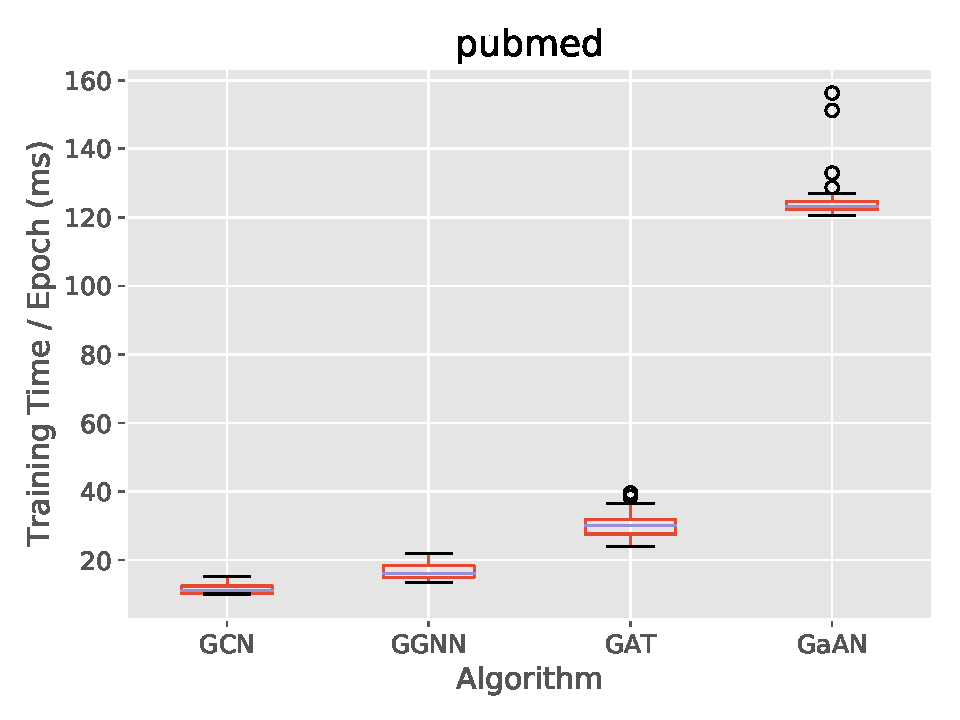
\includegraphics[height=4cm]{figs/experiments/exp_absolute_training_time_comparison_pubmed.pdf}}
    \subfloat[\texttt{aph}\label{fig:exp_absolute_training_time_amazon-photo}]{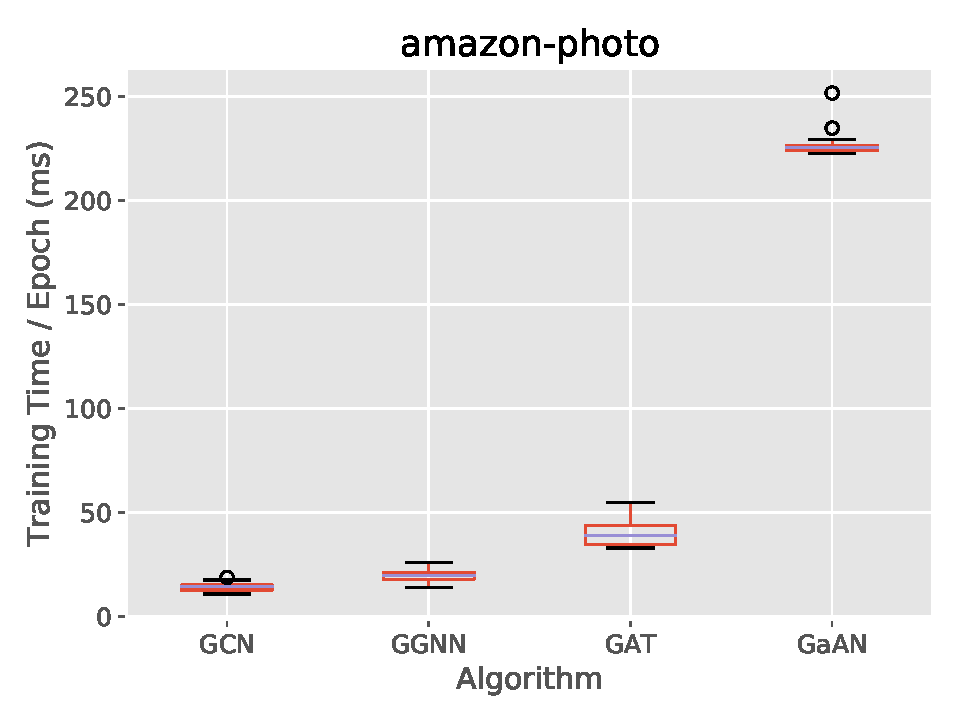
\includegraphics[height=4cm]{figs/experiments/exp_absolute_training_time_comparison_amazon-photo.pdf}}
    \subfloat[\texttt{cph}\label{fig:exp_absolute_training_time_coauthor-physics}]{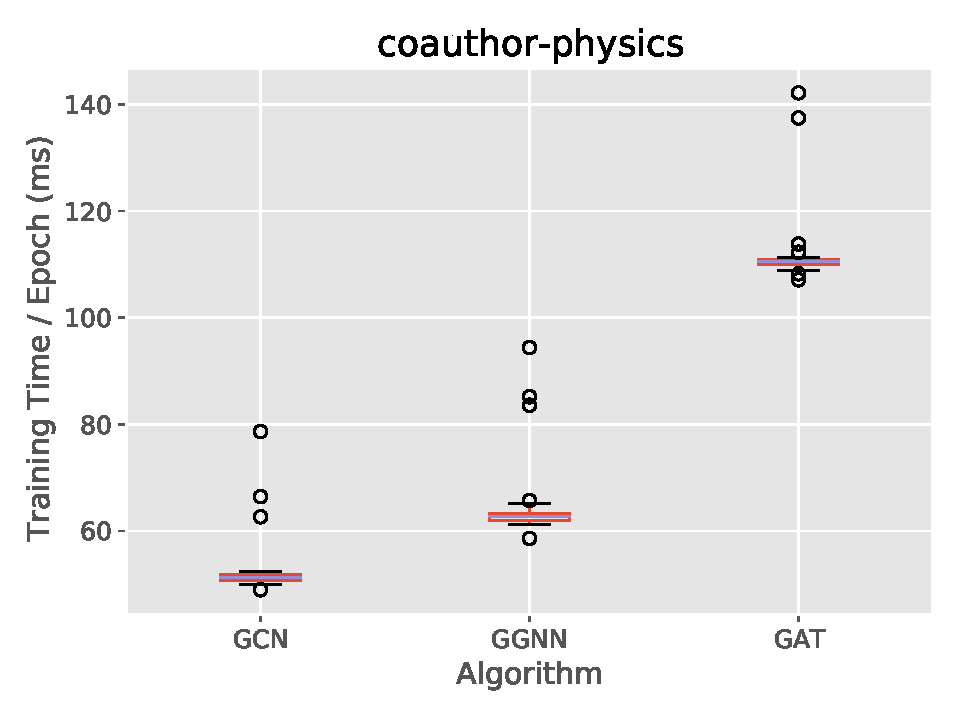
\includegraphics[height=4cm]{figs/experiments/exp_absolute_training_time_comparison_coauthor-physics.pdf}} \\
    \subfloat[\texttt{amc}\label{fig:exp_absolute_training_time_amazon-computers}]{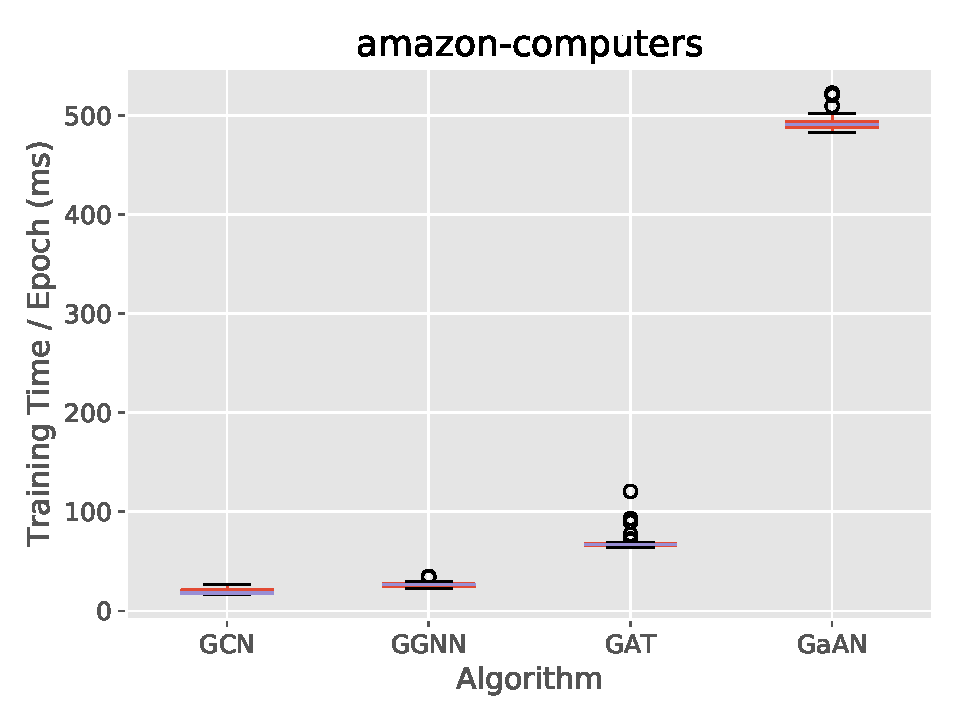
\includegraphics[height=4cm]{figs/experiments/exp_absolute_training_time_comparison_amazon-computers.pdf}}
    \subfloat[\texttt{fli}\label{fig:exp_absolute_training_time_flickr}]{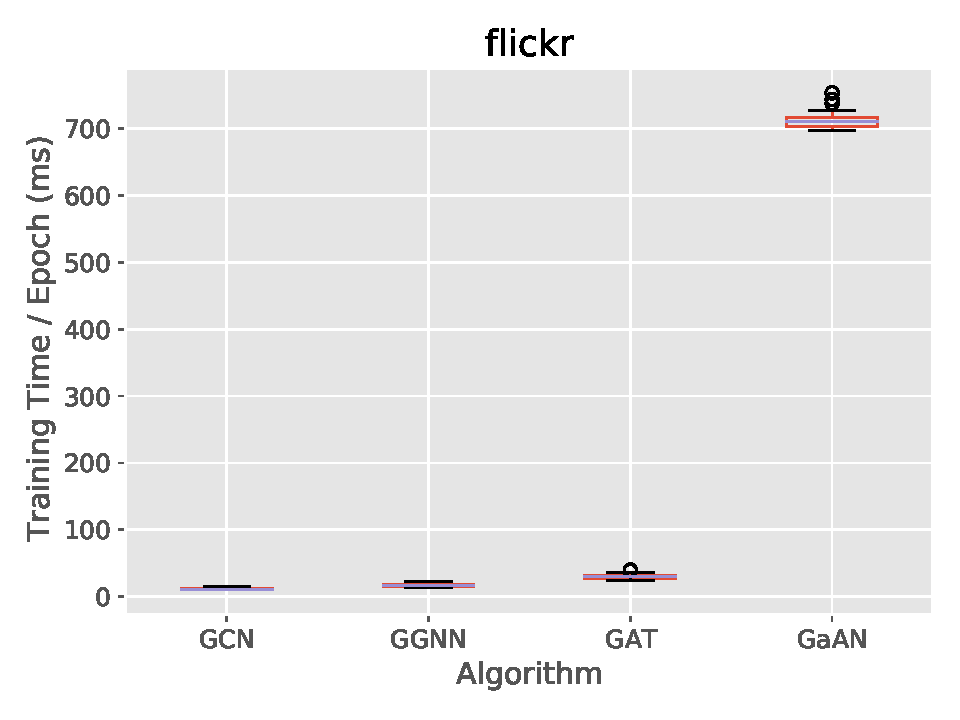
\includegraphics[height=4cm]{figs/experiments/exp_absolute_training_time_comparison_flickr.pdf}}
    \subfloat[\texttt{cam}\label{fig:exp_absolute_training_time_com-amazon}]{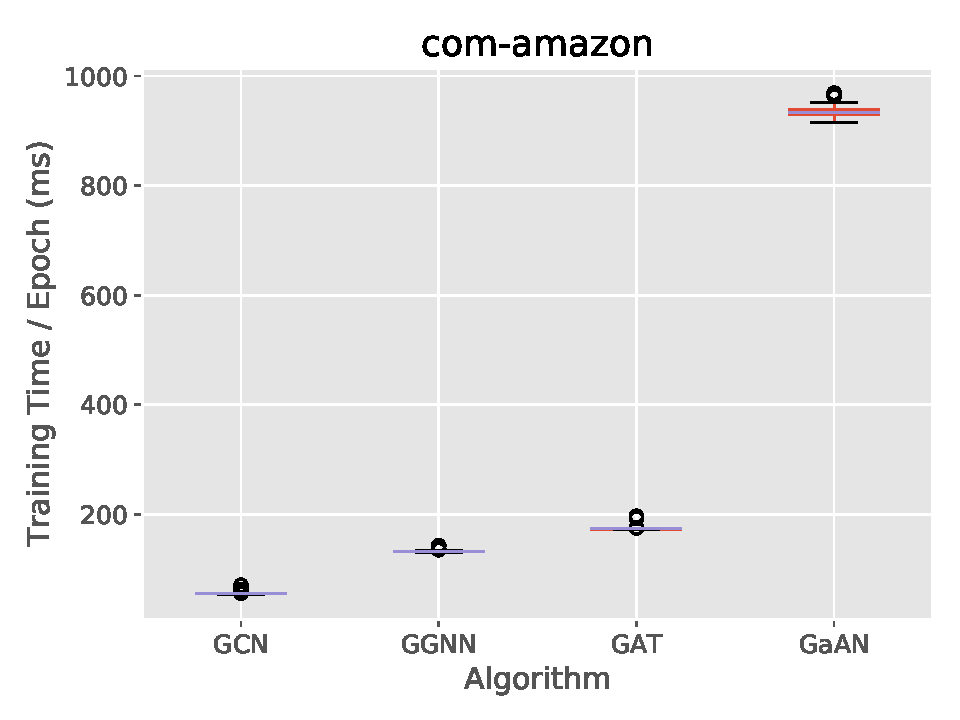
\includegraphics[height=4cm]{figs/experiments/exp_absolute_training_time_comparison_com-amazon.pdf}}
    \caption{Distribution of the wall-clock training time of 50 epoches on different datasets. GaAN crashed due to out of memory exception on the \texttt{cph} dataset.}
    \label{fig:exp_absolute_training_time}
\end{figure}

To further evaluate the effects of hyper-parameters, we measured the training time of each GNN with varying hyper-parameters in \figurename~\ref{fig:exp_hyperparameter_on_vertex_edge_phase_time}.

\begin{figure}
    \centering
    \subfloat[GCN\label{fig:exp_hyperparameter_on_vertex_edge_phase_time_gcn}]{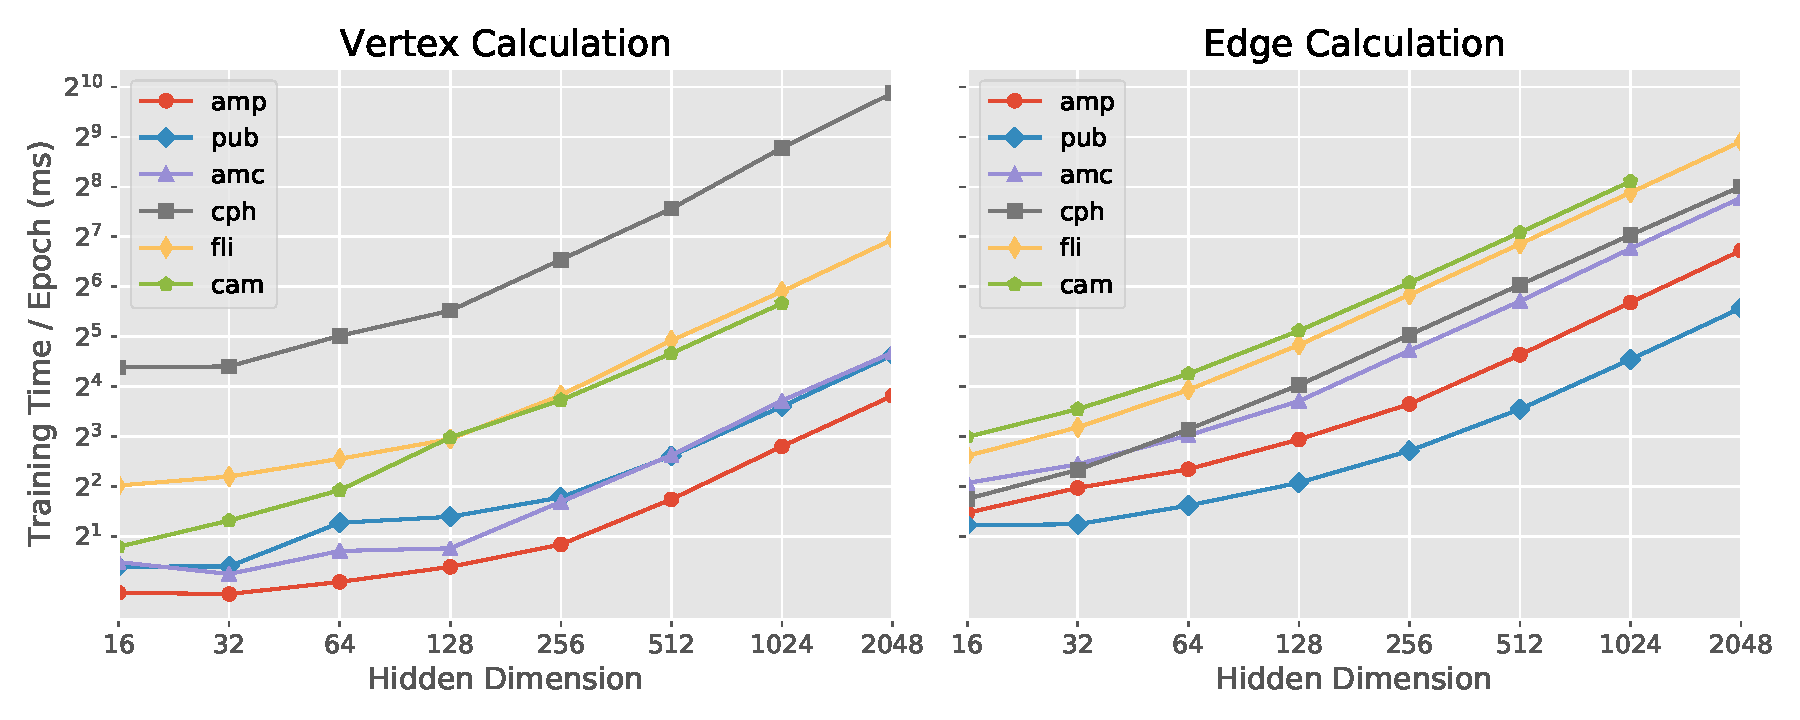
\includegraphics[height=3cm]{figs/experiments/exp_hyperparameter_on_vertex_edge_phase_time_gcn.pdf}}
    %
    \subfloat[GGNN\label{fig:exp_hyperparameter_on_vertex_edge_phase_time_ggnn}]{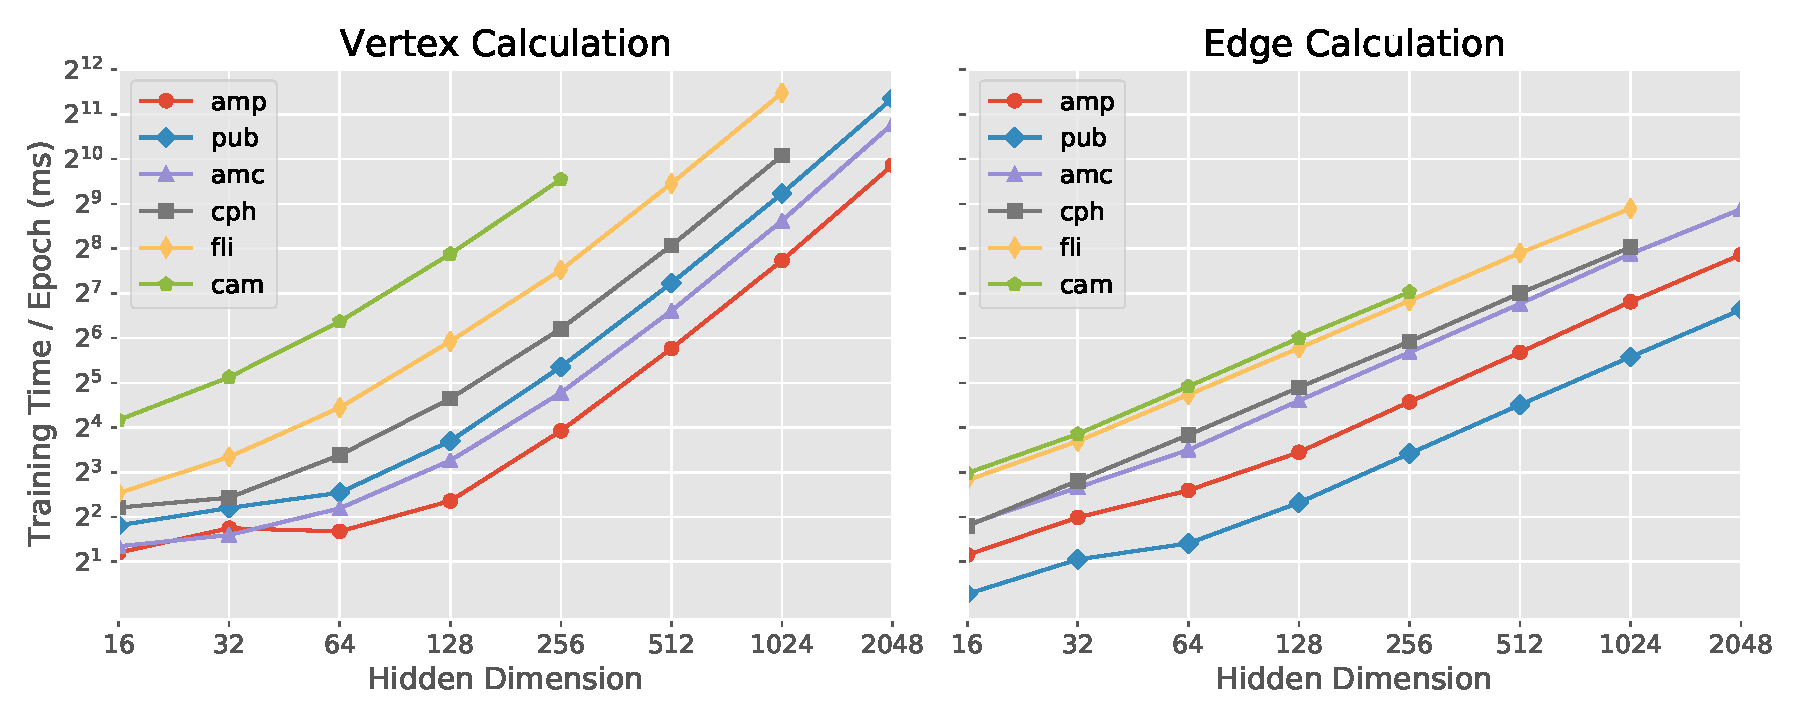
\includegraphics[height=3cm]{figs/experiments/exp_hyperparameter_on_vertex_edge_phase_time_ggnn.pdf}}
    \\
    \subfloat[GAT\label{fig:exp_hyperparameter_on_vertex_edge_phase_time_gat}]{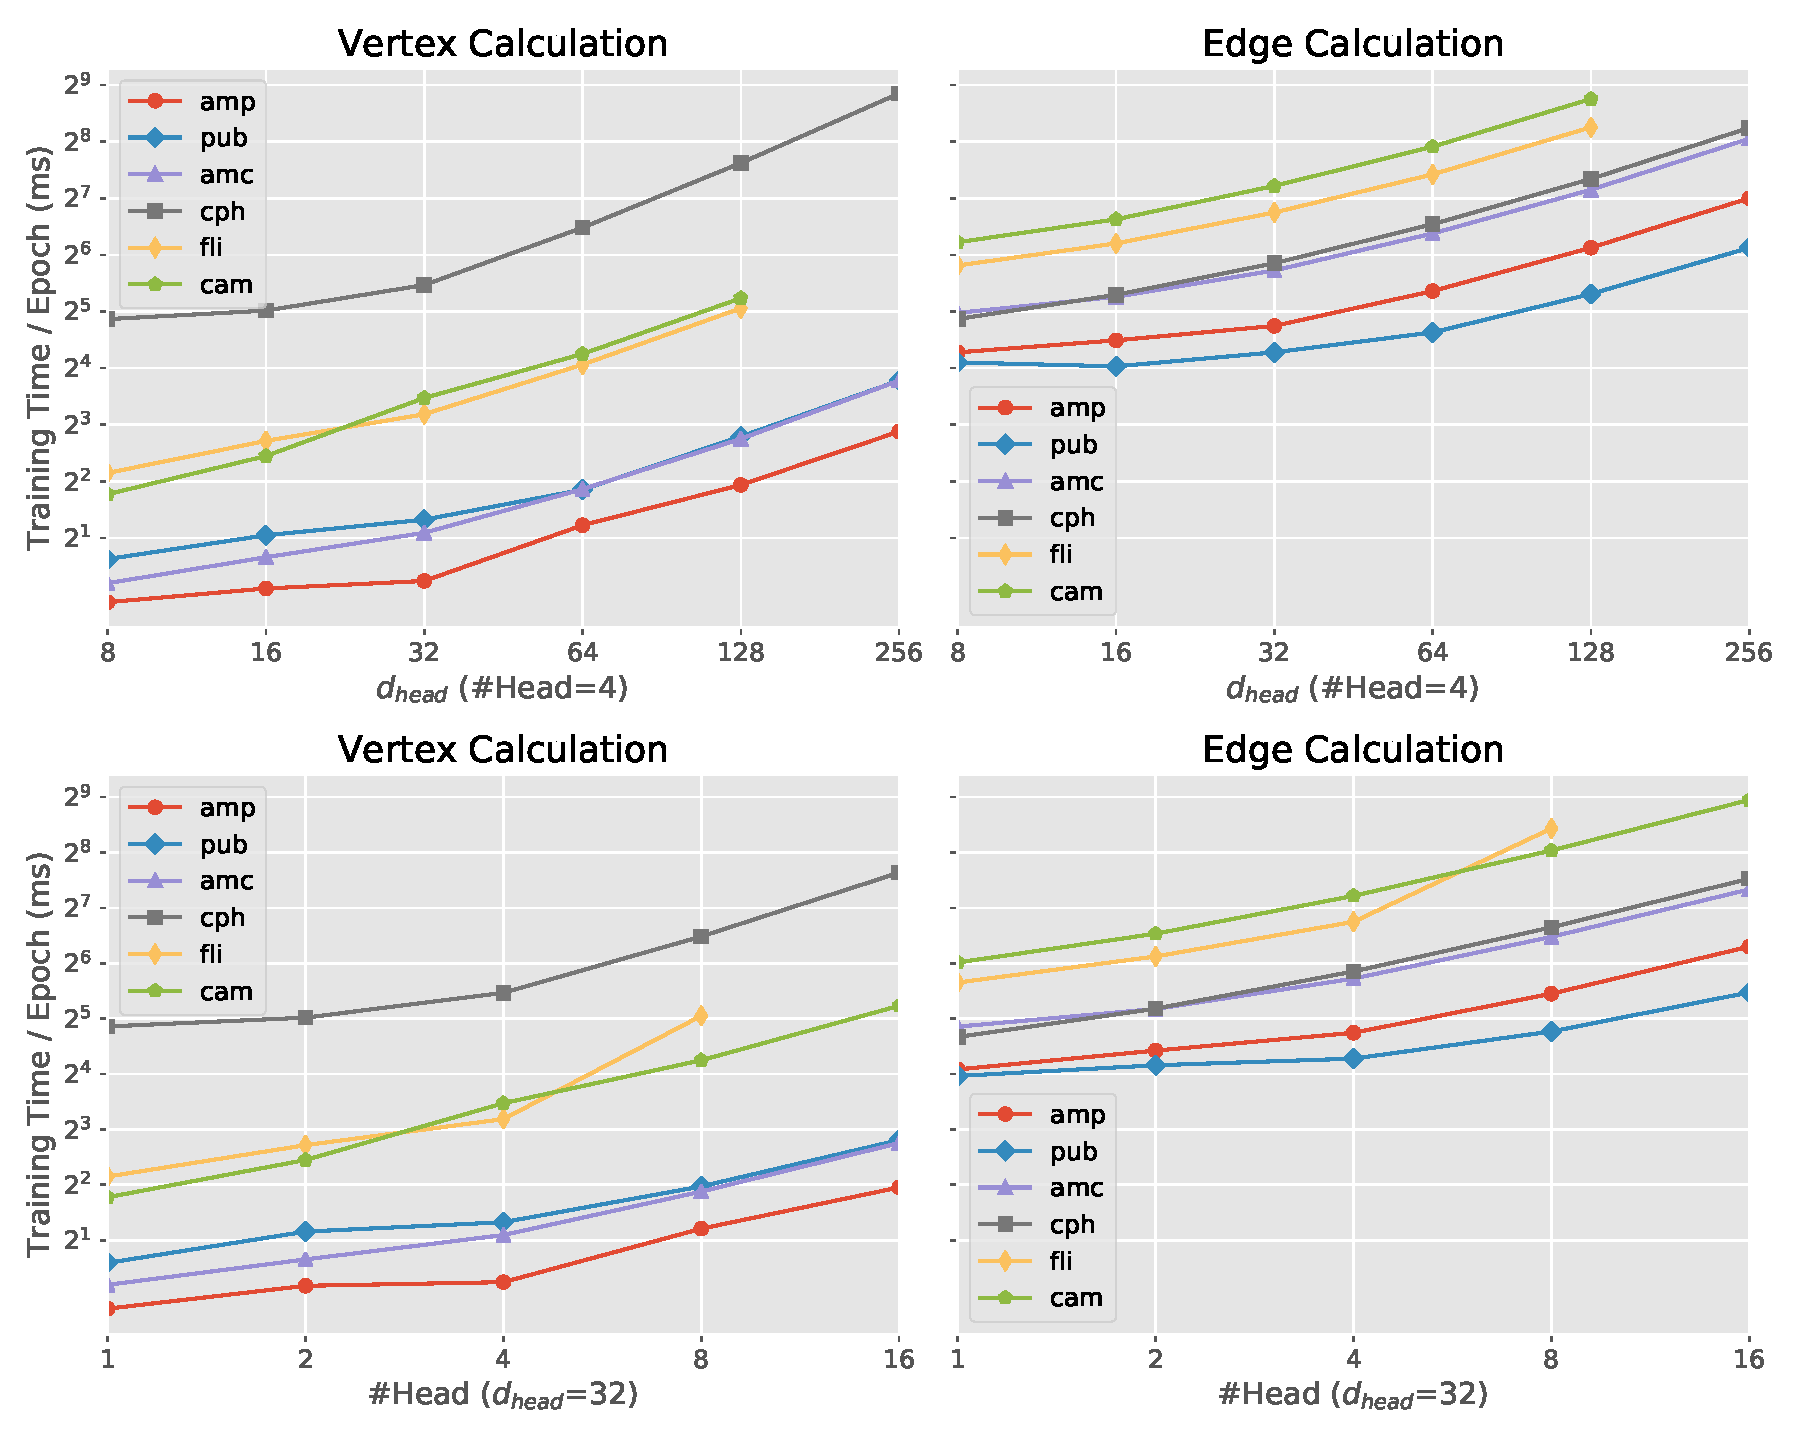
\includegraphics[height=6cm]{figs/experiments/exp_hyperparameter_on_vertex_edge_phase_time_gat.pdf}}
    \\
    \subfloat[GaAN\label{fig:exp_hyperparameter_on_vertex_edge_phase_time_gaan}]{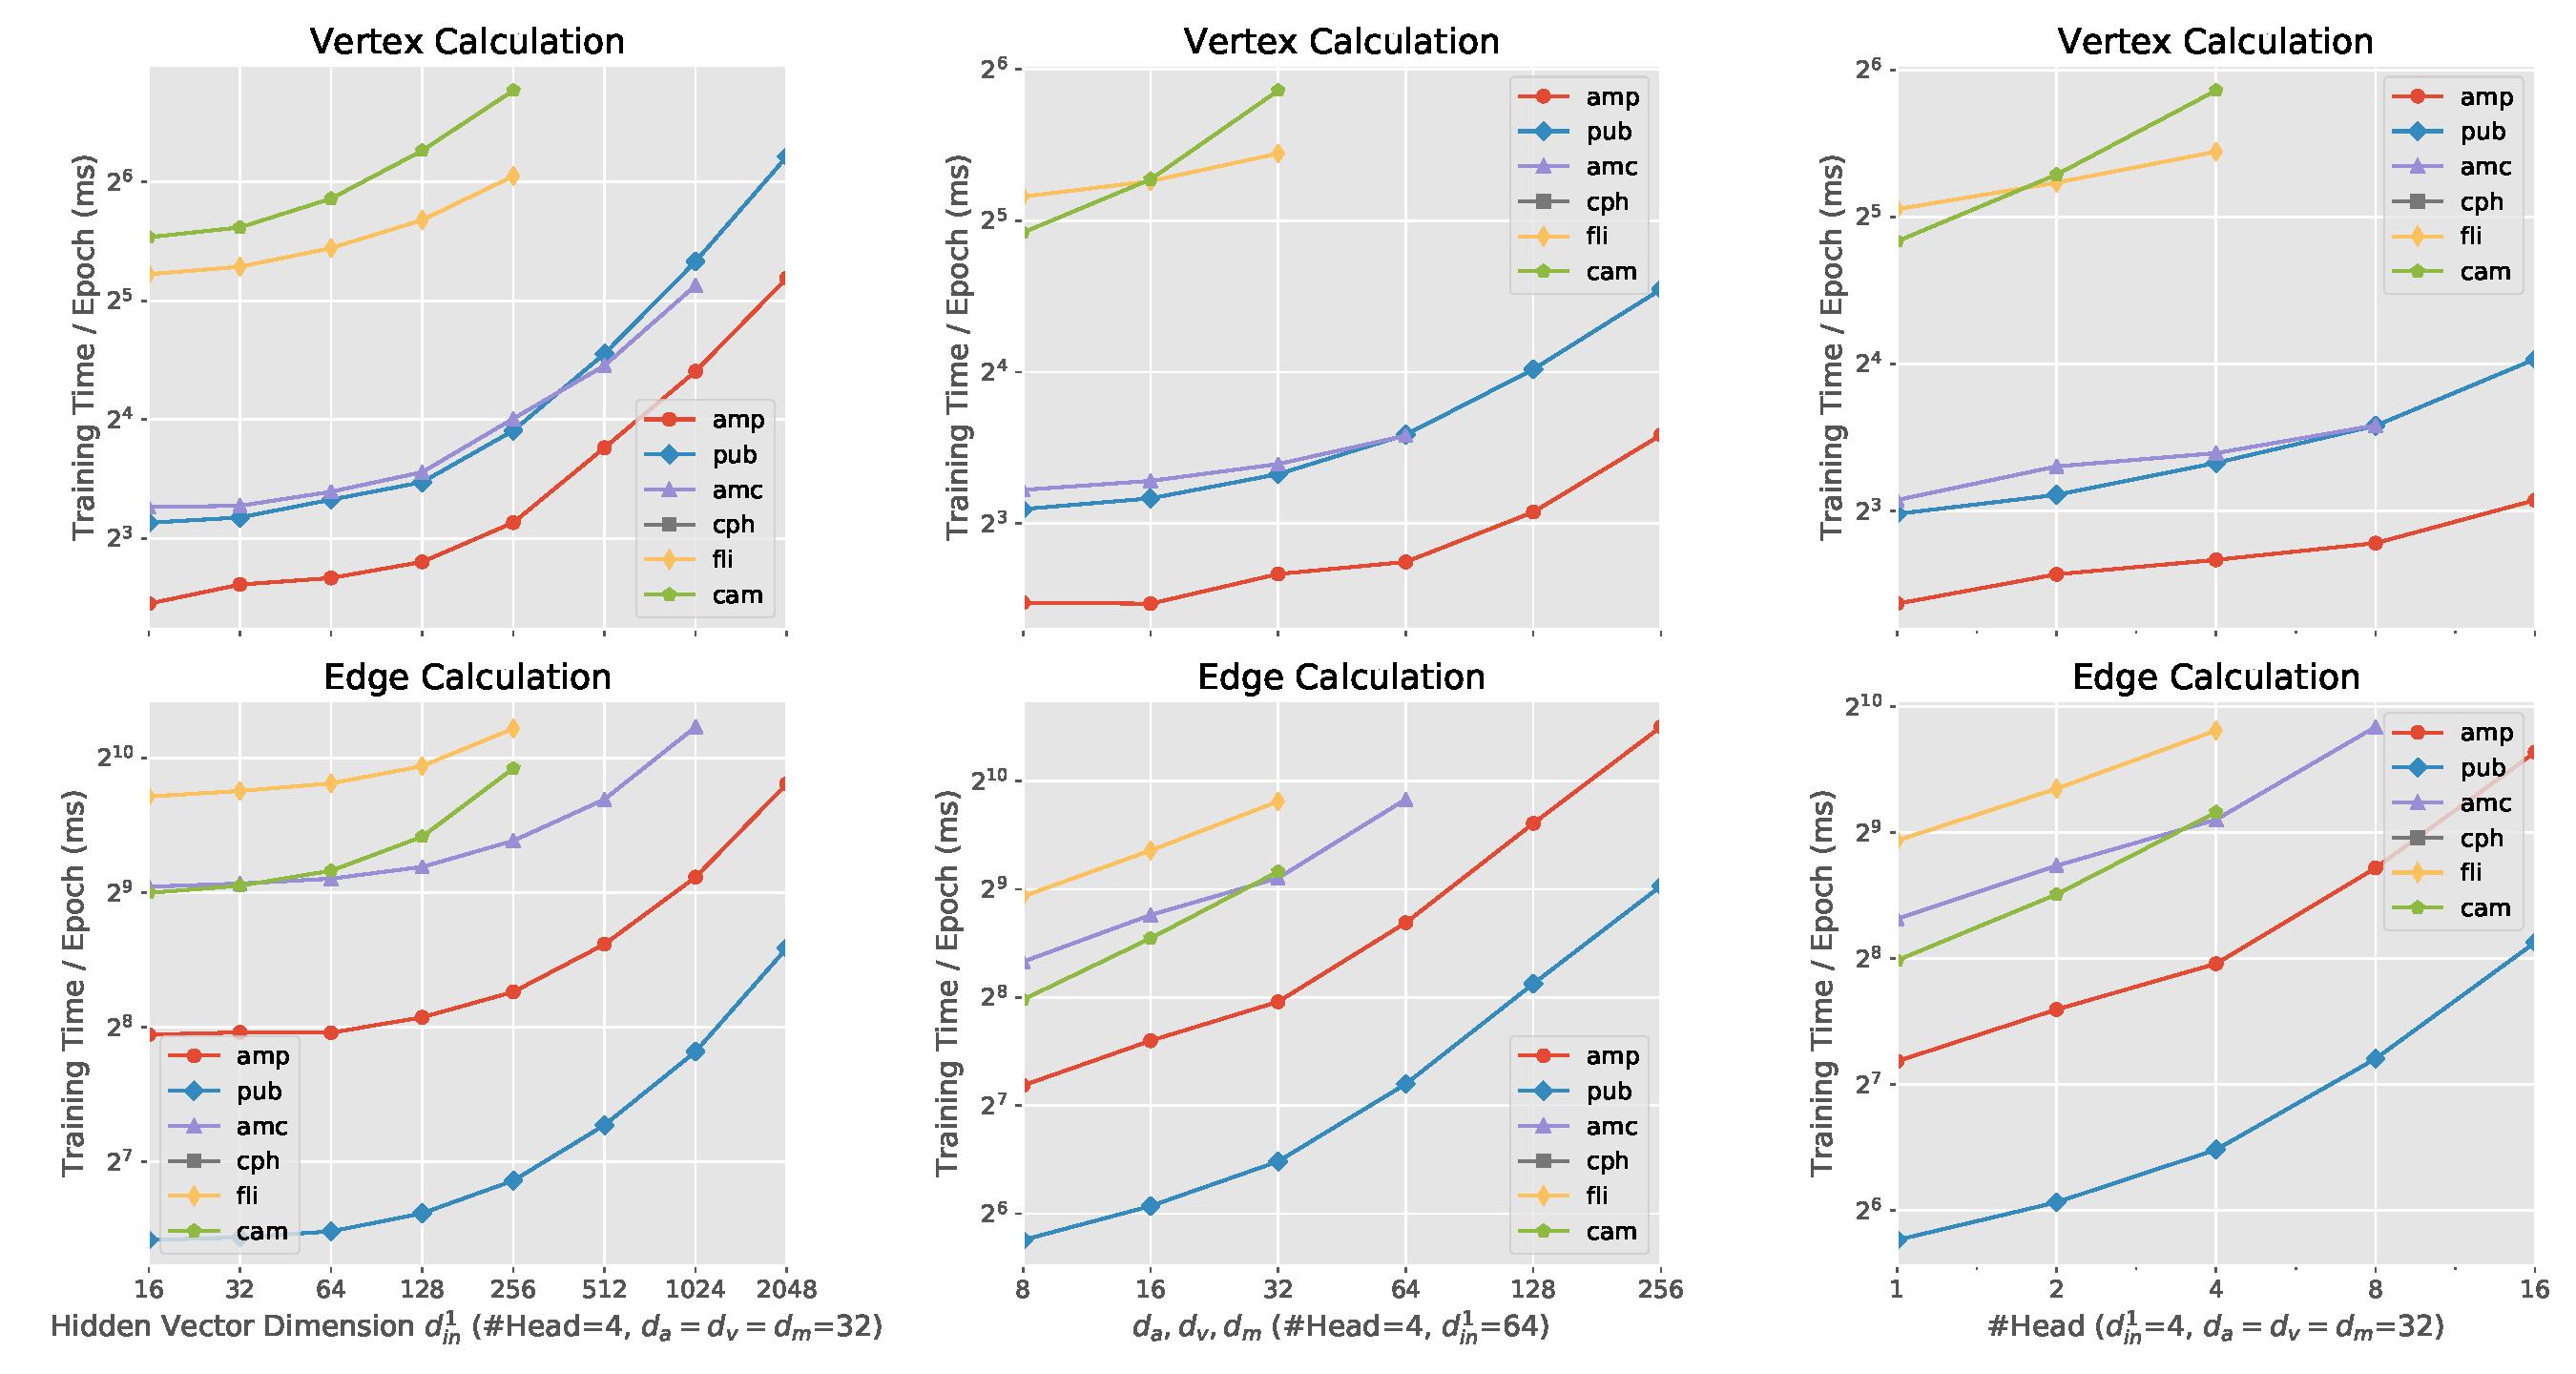
\includegraphics[height=6cm]{figs/experiments/exp_hyperparameter_on_vertex_edge_phase_time_gaan.pdf}}

    \caption{Effects of hyper-parameters on the vertex/edge calculation time.}
    \label{fig:exp_hyperparameter_on_vertex_edge_phase_time}
\end{figure}


For GCN and GGNN, the only modifiable hyper-parameter is the hidden dimension $dim(\boldsymbol{h}^1)$ with $dim(\boldsymbol{h}^1) = d^0_{out} = d^1_{in}$.
$dim(\boldsymbol{h}^0)$ and $dim(\boldsymbol{h}^2)$ is determined by the dataset with $dim(\boldsymbol{h}^0)=dim(\boldsymbol{x})$ and $dim(\boldsymbol{h}^2)=$\#Classes.
\figurename~\ref{fig:exp_hyperparameter_on_vertex_edge_phase_time_gcn} and \figurename~\ref{fig:exp_hyperparameter_on_vertex_edge_phase_time_ggnn} show that the training time of GCN and GGNN increased linearly under big $dim(\boldsymbol{h}^1)$, consistent with the time complexity analysis.

For GAT, we modified the number of heads $K$ and the dimension of each head $d_{head}$ in the GAT layer 0.
The dimenstion of the hidden feature vector was determined correspondingly as $d^0_{out} = d^1_{in} = dim(\boldsymbol{h}^1) = K h_{head}$.
\figurename~\ref{fig:exp_hyperparameter_on_vertex_edge_phase_time_gat} shows that the GAT training time increases linearly under big $d_{head}$ and $K$.

For GaAN, it is also based on the multi-head mechanism.
Its time complexity is affected by $d_{in}$, $d_v$, $d_a$ and the number of heads $K$.
\figurename~\ref{fig:exp_hyperparameter_on_vertex_edge_phase_time_gaan} demonstrates that the training time increased linearly with the hyper-parameters, except for $dim(\boldsymbol{h}^1)$.
As $dim(\boldsymbol{h}^1)$ increased, the training time increased first slightly and then linearly.
We could observe similar phenomena in GCN, GGNN and GAT with low hyper-parameters.
When the hyper-parameter was too low, the GNN training could not make use of the full computing power of the GPU.
When it became high enough, the training time increased linearly.

\begin{figure}
    \centering
    \subfloat[GCN]{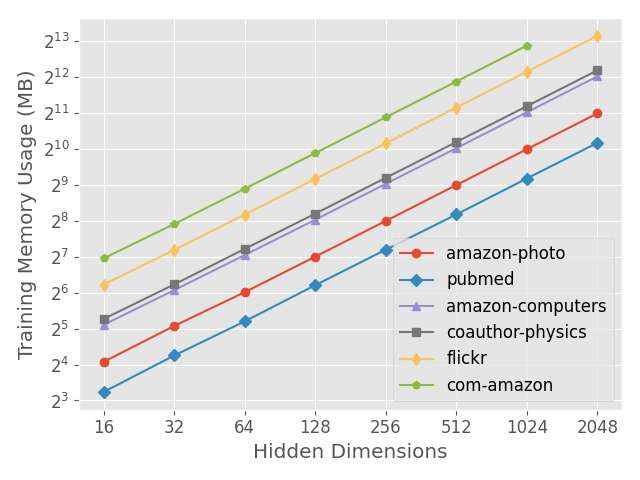
\includegraphics[height=3cm]{figs/experiments/exp_hyperparameter_on_memory_usage_gcn.png}}
    \subfloat[GGNN]{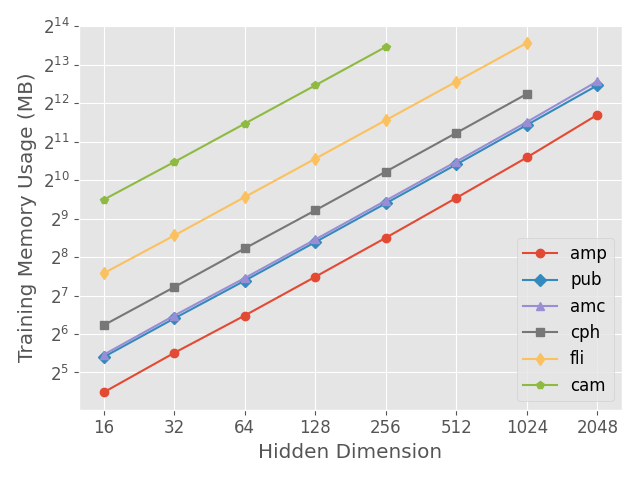
\includegraphics[height=3cm]{figs/experiments/exp_hyperparameter_on_memory_usage_ggnn.png}}\\
    \subfloat[GAT]{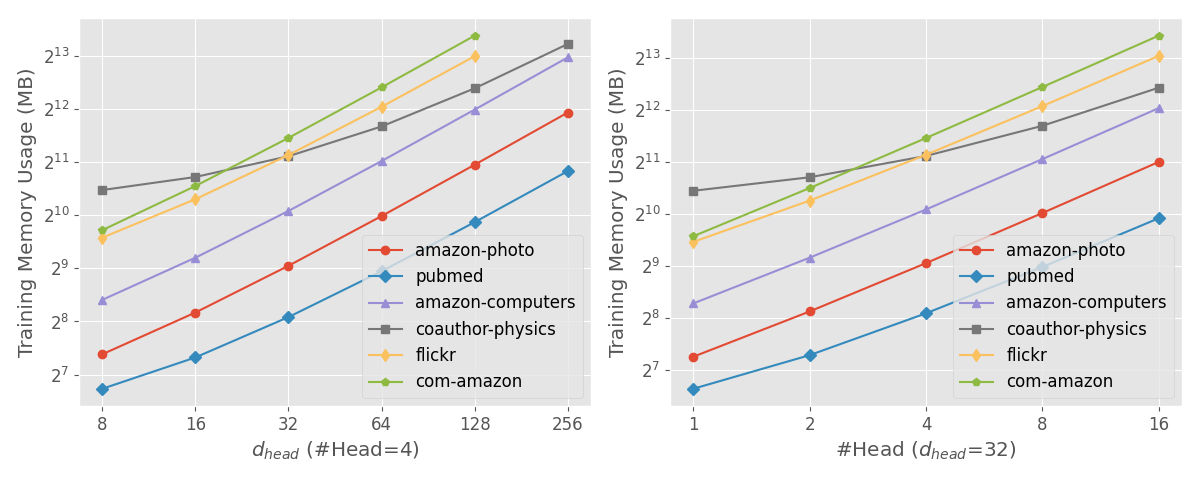
\includegraphics[height=3cm]{figs/experiments/exp_hyperparameter_on_memory_usage_gat.png}}\\
    \subfloat[GaAN]{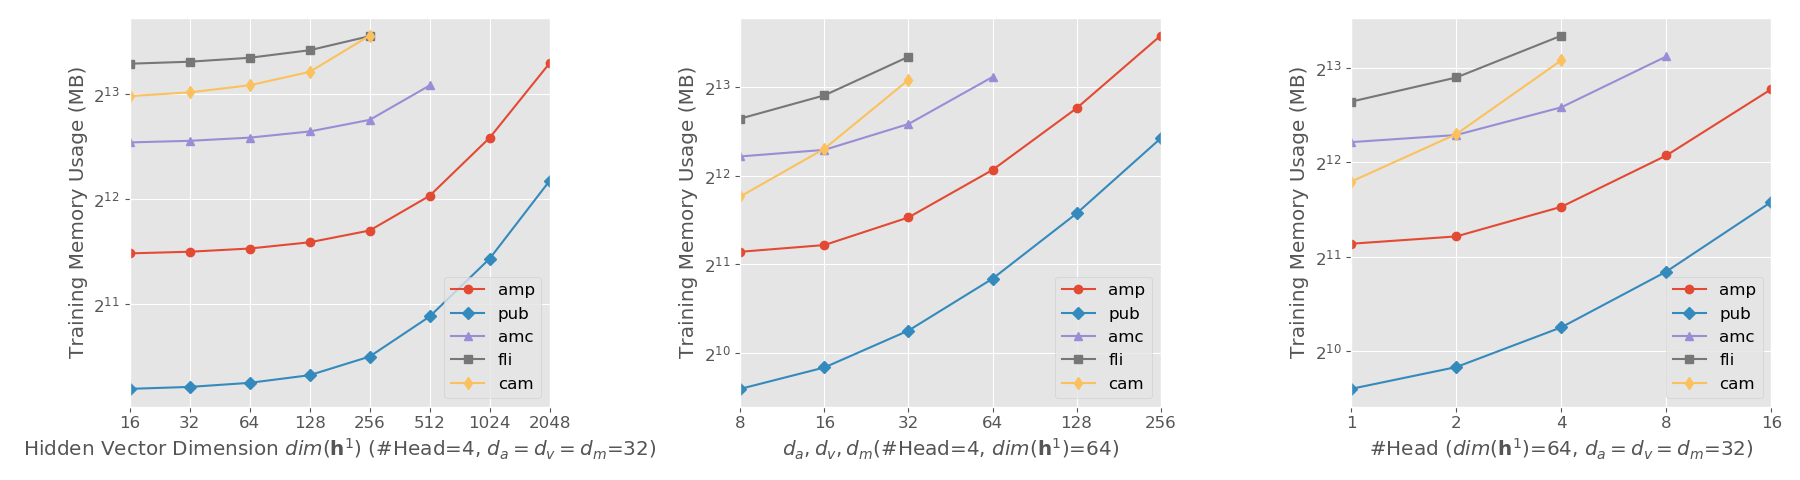
\includegraphics[height=3cm]{figs/experiments/exp_hyperparameter_on_memory_usage_gaan.png}}
    \caption{Effects of hyper-parameters on the peak GPU memory usage during the training, excluding the memory used by the dataset and the model parameters.}
    \label{fig:exp_hyperparameter_memory_usage}
\end{figure}

The experimental results support the time complexity analysis.
We further measured the effects of the hyper-parameters on the peak GPU memory usage in \figurename~\ref{fig:exp_hyperparameter_memory_usage}.
The memory usage also increased linearly as the hyper-parameters increased for all GNNs, except for GaAN on $dim(\boldsymbol{h}^1)$.
As the hidden feature vectors $\boldsymbol{h}^1$ consumed a small proportion of memory in GaAN, the growth in the memory usage was not noticable until $dim(\boldsymbol{h}^1)$ was large enough.

\paragraph{Summary}

The complexity analysis in \tablename~\ref{tab:gnn_overview_edge} and \tablename~\ref{tab:gnn_overview_vertex} is valid.
The hyper-parameters affect the training time and the memory usage of the GNN training \textbf{in a linear way}.
Algorithm enginners can use larger hyper-parameters to increase the expressive power of a GNN model without worrying the explosive growth in the training time and memory usage.

\subsection{Training Time Breakdown}
\label{sec:training_time_breakdown}

To find out which stage/step dominates the training time, we breakdown the training time and analyze the performance bottleneck level by level.

\subsubsection{Layer Level}

\begin{figure}
    \centering
    \subfloat[GCN]{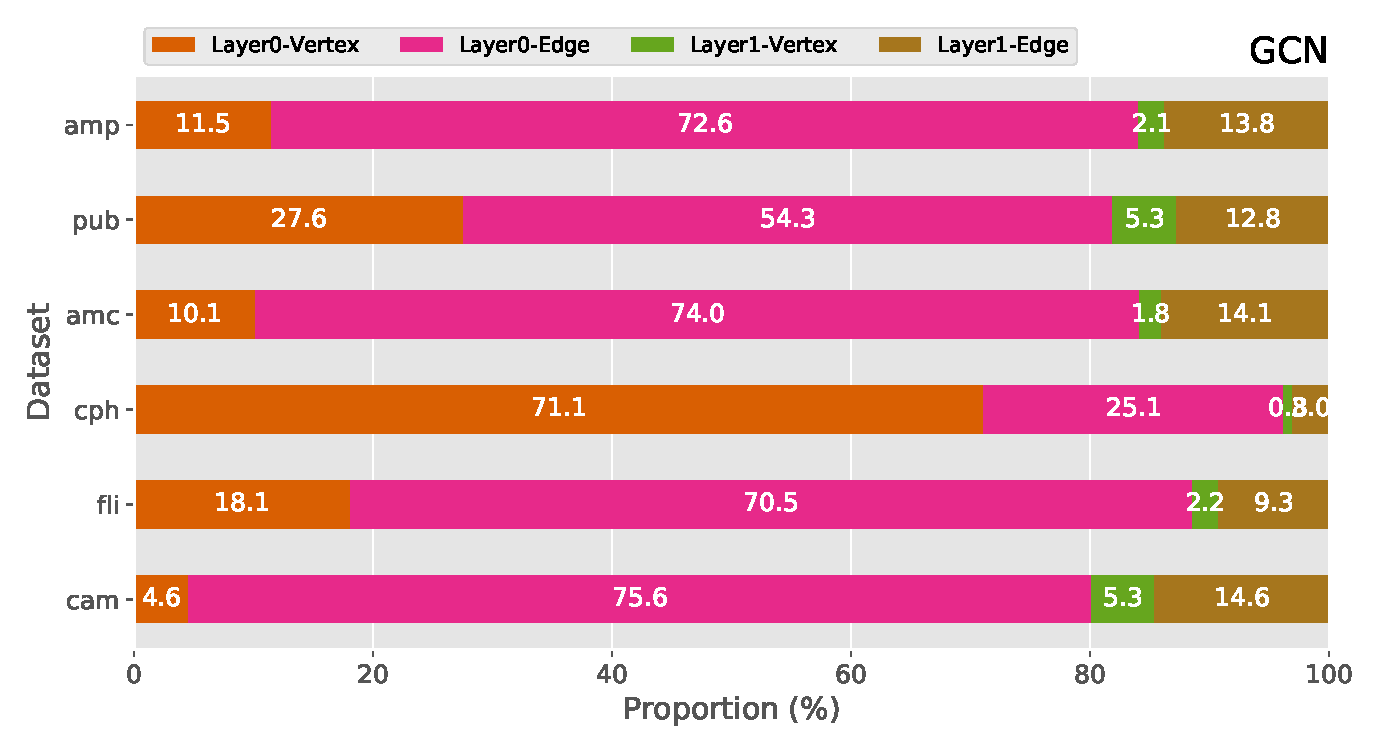
\includegraphics[height=4cm]{figs/experiments/exp_layer_time_proportion_gcn.pdf}}
    \subfloat[GGNN]{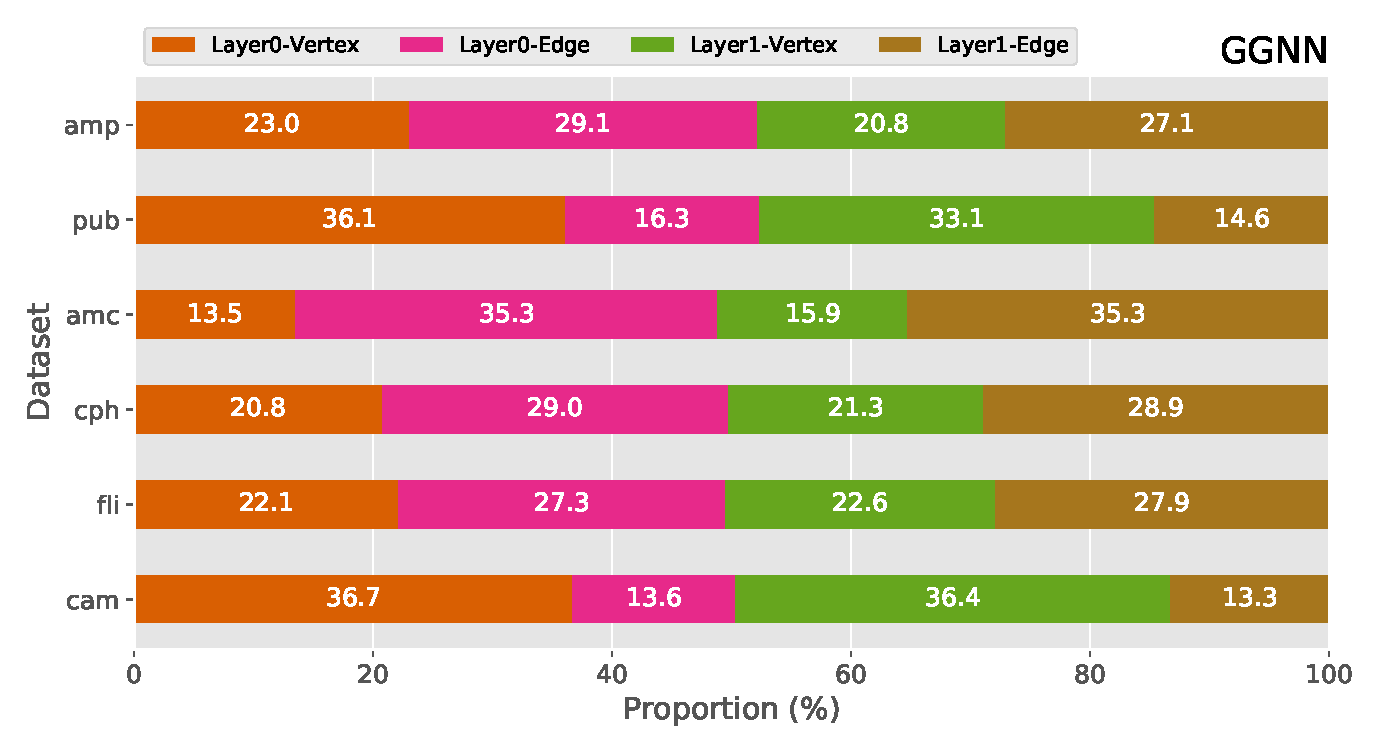
\includegraphics[height=4cm]{figs/experiments/exp_layer_time_proportion_ggnn.pdf}}\\
    \subfloat[GAT]{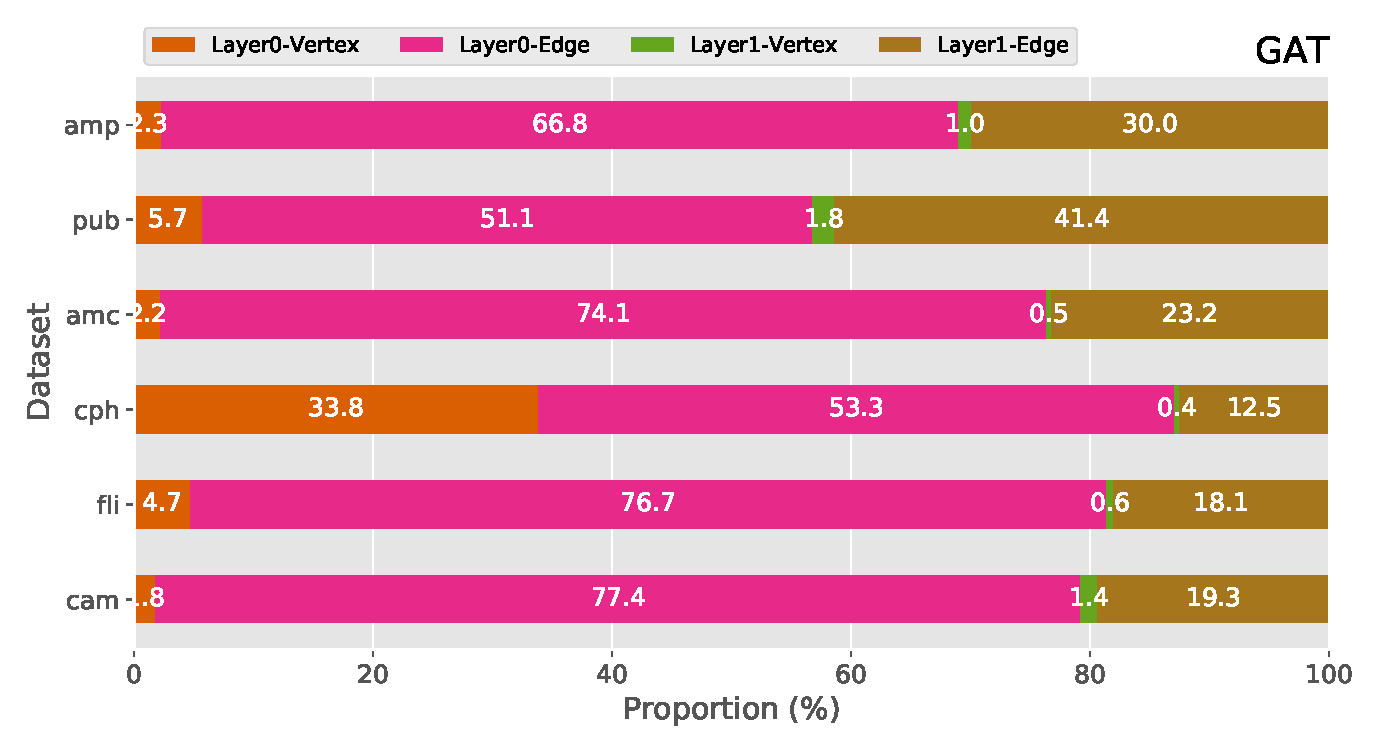
\includegraphics[height=4cm]{figs/experiments/exp_layer_time_proportion_gat.pdf}}
    \subfloat[GaAN]{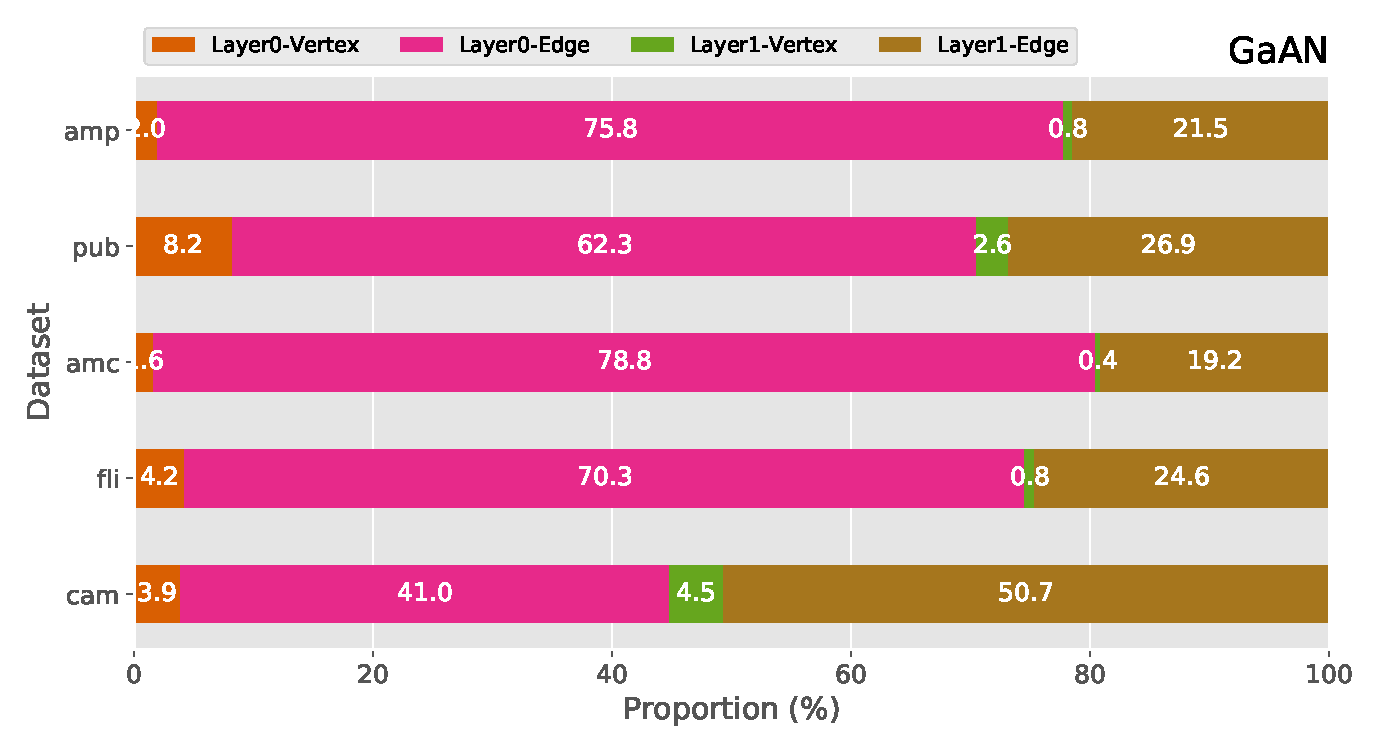
\includegraphics[height=4cm]{figs/experiments/exp_layer_time_proportion_gaan.pdf}}
    \caption{Training time breakdown on the layer level. The training time of each layer includes the time spent on the forward, backward and evaluation phases. Each layer is further decomposed into the vertex and the edge calculation stages.}
    \label{fig:exp_vertex_edge_cal_proportion}
\end{figure}

\figurename~\ref{fig:exp_vertex_edge_cal_proportion} decomposes the training time of a GNN on the layer level.
The training time of each layer is the summation of the time in the forward, backward and evaluation phases.
In GCN, GAT and GaAN, the time spent on the layer 0 was much larger than the layer 1.
In those GNNs, the dimensions of the input/output feature vectors in the layer 0 were much larger than the dimensions in the layer 1.
$d^0_{in}=dim(\boldsymbol{x})$, $d^0_{out}=d^1_{in}=64$ and $d^1_{out}=\#Class$ and $dim(\boldsymbol{x}) \gg \#Class$.
For GaAN, since it required the dimensions of the input/output feature vectors must be same, $d^0_{in}=d^0_{out}=d^1_{in}=d^1_{out}=64$ and the training time of both layers were close.

Each GNN layer can be further divided in the vertex and the edge calculation stages.
In \figurename~\ref{fig:exp_vertex_edge_cal_proportion}, GCN spent most of the training time on the edge calculation in most datasets.
A special case is \texttt{cph} dataset.
The dimension of the input feature vectors was very high in \texttt{cph}, making the vertex calculation stage of the GCN Layer 0 spend considerable time.
GGNN also spent the majority of its training time on the edge calculation.
But the high time complexity of its vertex update function $\gamma$ made the ratio of the vertex calculation in the total training time much higher than other GNNs.
%In \textit{pub} and cam dataset, the edge calculation cost and the vertex calculation cost are close for GGNN
%because the average degree of the two datasets is low (only 4.5 and 2.8).
For GAT and GaAN, due to their high edge calculation complexity, the edge calculation is the absolutely dominant stage.
In summary, \emph{the edge calculation is the most time-consuming stage in the GNN training}.

\begin{figure}
    \centering
    \subfloat[GCN]{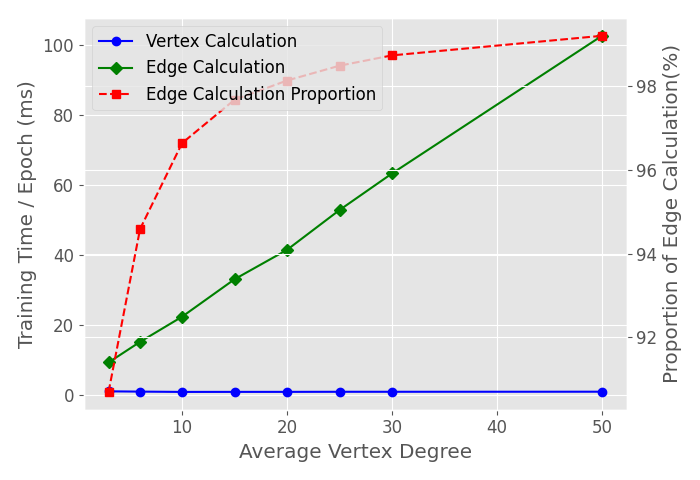
\includegraphics[height=4cm]{figs/experiments/exp_avg_degree_on_vertex_edge_cal_time_gcn.png}}
    \subfloat[GGNN]{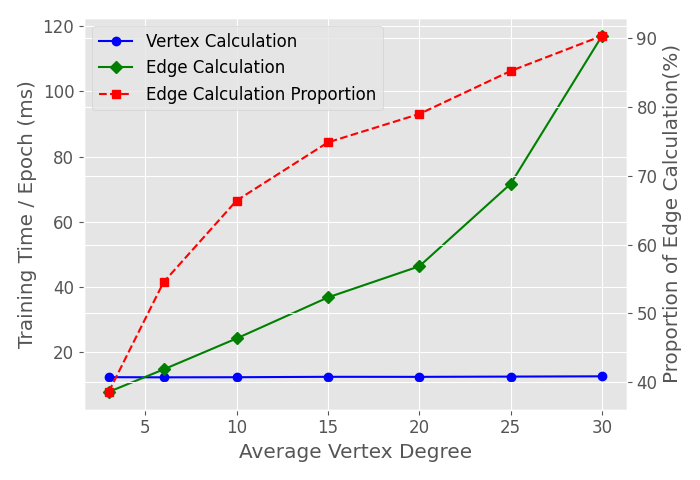
\includegraphics[height=4cm]{figs/experiments/exp_avg_degree_on_vertex_edge_cal_time_ggnn.png}}\\
    \subfloat[GAT]{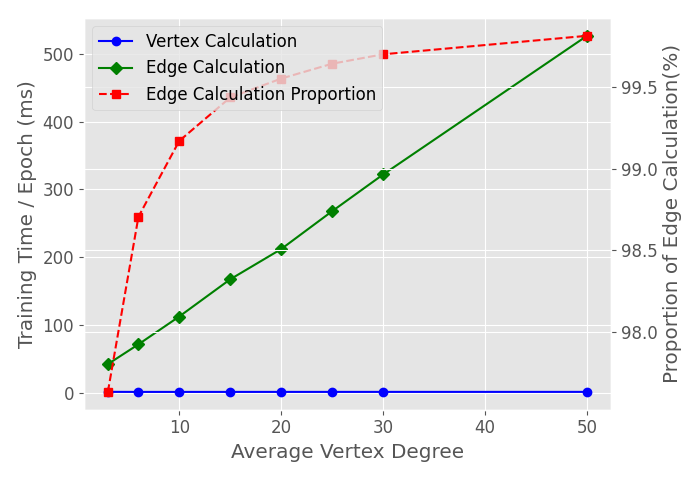
\includegraphics[height=4cm]{figs/experiments/exp_avg_degree_on_vertex_edge_cal_time_gat.png}}
    \subfloat[GaAN]{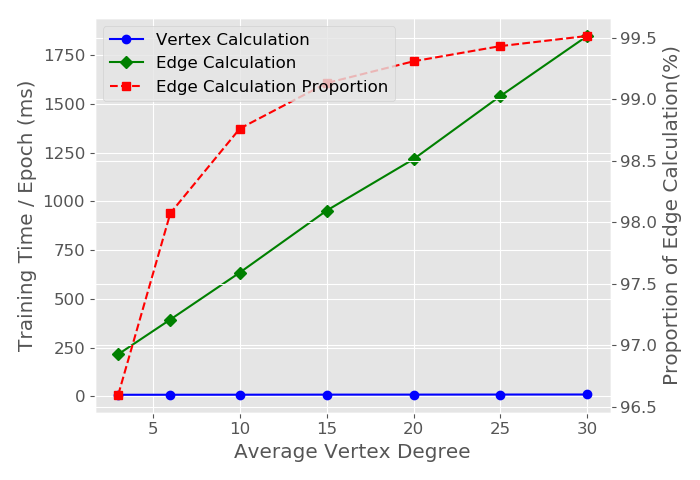
\includegraphics[height=4cm]{figs/experiments/exp_avg_degree_on_vertex_edge_cal_time_gaan.png}}
    \caption{Effects of the average degree on the time proportion of the vertex/edge calculation. Graphs were generated with the R-MAT generator by fixing the number of vertices as 50,000. }
    \label{fig:exp_avg_degree_on_vertex_edge_cal_time}
\end{figure}

The experimental results also indicate that the average degree of the dataset affects the time-consuming proportion of the vertex/edge calculation.
For GaAN, the time spent on the vertex calculation exceeded the edge calculation on the \texttt{pub} and \texttt{cam} datasets, because the avaerage degrees of the two datasets were low, making $|\mathcal{E}|$ and $|\mathcal{V}|$ much closer.
To evaluate the effects of the average degree, we used the R-MAT model to generate random graphs with 50k vertices and the average degrees ranging from 2 to 100.
\figurename~\ref{fig:exp_avg_degree_on_vertex_edge_cal_time} shows the training time of the four GNNs under different average degrees.
As the average degree increased, the training time of the edge calculation grew \emph{linearly}.
For GCN, GAT and GaAN, the edge calculation dominated the entire training time even under small average degrees.
Only for GGNN that had high vertex and low edge calculation complexities, the training time of the vertex calculation could exceed the edge calculation under low average degrees ($<5$).
Therefore, \emph{improving the efficiency of the edge calculation is the key to reduce the GNN training time}.

\subsubsection{Step Level in Edge Calculation}

\begin{figure}
    \centering
    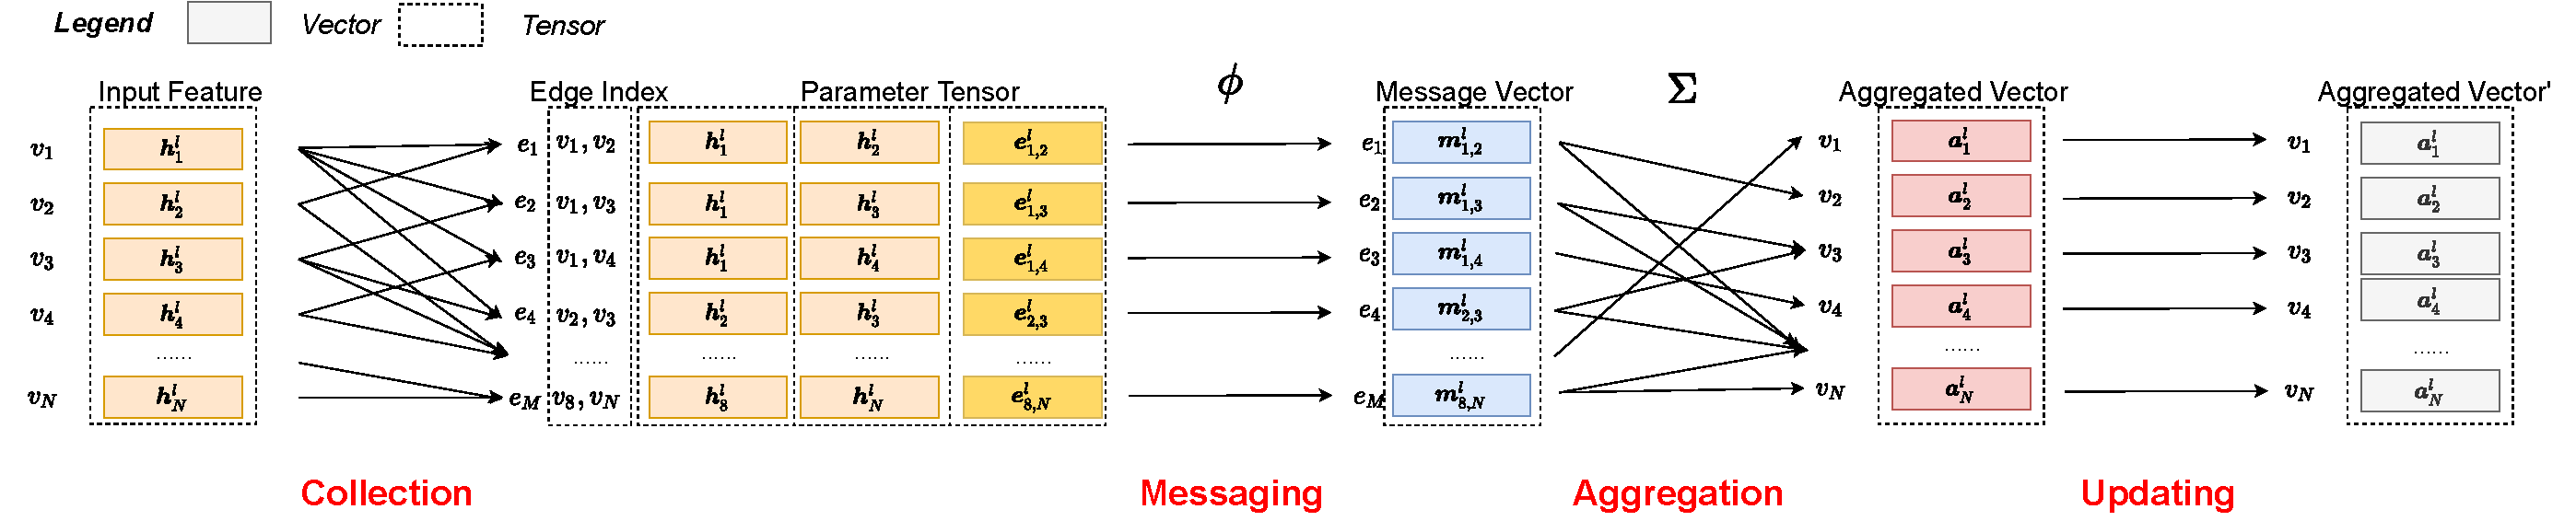
\includegraphics[width=1\columnwidth]{figs/illustration/steps_in_edge_calculation.pdf}
    \caption{Step decomposition of the edge calculation in the GNN layer $l$.}
    \label{fig:steps_in_edge_calculation}
\end{figure}

In the implementation of PyG, the edge calculation stage can be decomposed into four steps: collect, message, aggregate and update, as shown in \figurename~\ref{fig:steps_in_edge_calculation}.
The edge index is a matrix with $M$ rows and 2 columns that holds the edge set of the graph, where $M=|\mathcal{E}|$.
The two columns of the matrix store the source vertex and the target vertex of each edge, respectively.
The collect step copies the vertex feature vectors from the previous layer $\boldsymbol{h}_i^l$ to the ends of each edge
in the edge index, to form the parameters $[\boldsymbol{h}^l_i, \boldsymbol{h}^l_{j}, \boldsymbol{e}^l_{i,j}]$ of the message function $\phi$.
This step only involves the data movement.
The message step calls the message function $\phi$ to get message vectors of all edges $\boldsymbol{m}_{i, j}^l$.
The aggregate step aggregates the message vectors with the same target vertex into a aggregated vector $\boldsymbol{s}^l_i$ with the aggregation operation $\Sigma$.
The update step is optinal.
It performs additional transformation on the aggregated vectors (for example, adding bias in GCN).
The aggregated vectors $\boldsymbol{s}^l_i$ (after the update step) will be fed into the vertex update function $\gamma$ as one of the input parameters.

\begin{figure}
    \centering
    \subfloat[GCN]{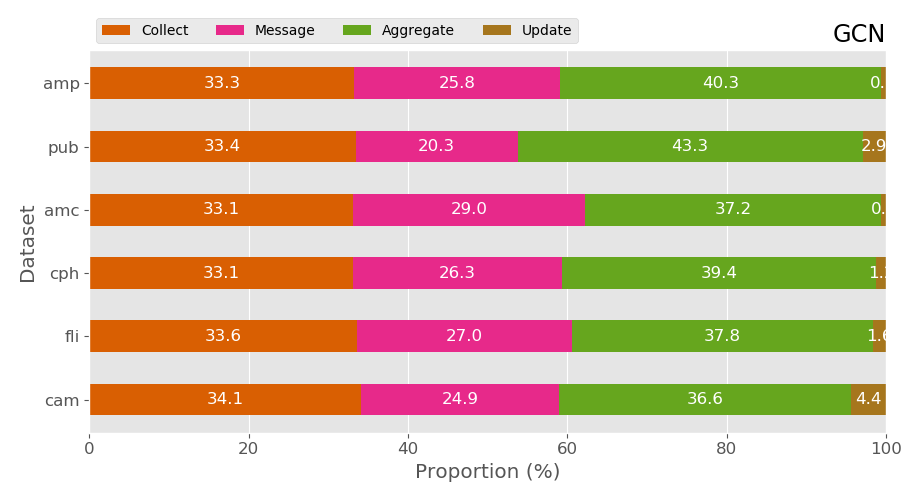
\includegraphics[height=4cm]{figs/experiments/exp_edge_calc_decomposition_gcn.png}}
    \subfloat[GGNN]{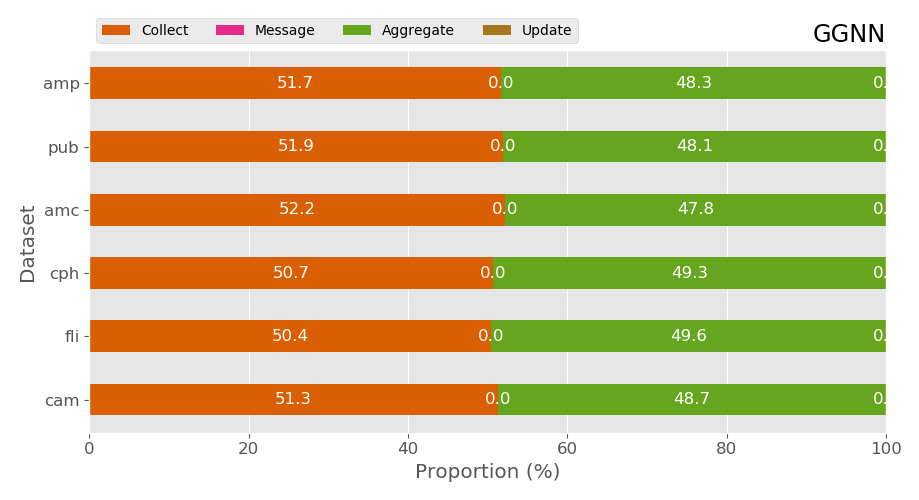
\includegraphics[height=4cm]{figs/experiments/exp_edge_calc_decomposition_ggnn.png}}\\
    \subfloat[GAT]{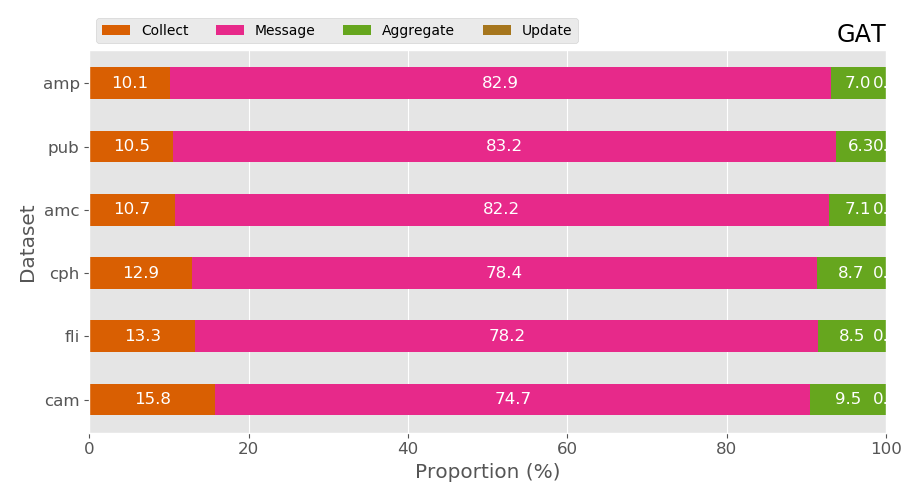
\includegraphics[height=4cm]{figs/experiments/exp_edge_calc_decomposition_gat.png}}
    \subfloat[GaAN]{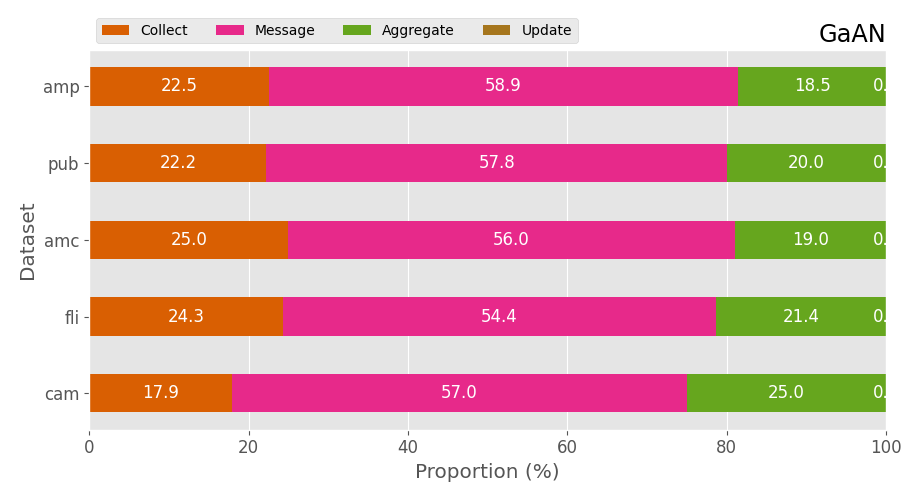
\includegraphics[height=4cm]{figs/experiments/exp_edge_calc_decomposition_gaan.png}}
    \caption{Training time breakdown of the edge calculation stage (including both GNN layers).}
    \label{fig:exp_edge_calc_decomposition}
\end{figure}

We decomposed the execution time of the edge calculation step in \figurename~\ref{fig:exp_edge_calc_decomposition}.
In each GNN, the proportion of the four steps were rather stable, rarely affected by datasets.
For GAT and GaAN with the high edge calculation complexity, the message step consumed most of the execution time.
For GCN and GGNN with the low complexity, the proportions of the steps were close.
Since the message function $\phi$ of GGNN used the pre-computed $\hat{\boldsymbol{h}}^l_i$ as the message vector directly in the implementation, the time spent on the message step of GGNN was negligible.
Although the collect step did not conduct any computation and only involved data movement, it occupied noticeable execution time in all the GNNs.
The experiments show that \emph{the performance bottleneck on the step level depends on the complexity of the edge calculation}.
For GNNs with the high edge calculation complexity, the message function $\phi$ is the performance bottleneck.
Optimizing its implementation can significantly reduce the training time.
For the other GNNs, optimization should focus on reducing the costs of the collect and the aggregation steps.
Addtionally, improving the efficiency of the collect step can benefit all GNNs.

\subsubsection{Operator Level}

The functions $\phi$, $\Sigma$ and $\gamma$ in the vertex and edge calculation are made up of a series of basic operators implemented on GPU, like the matrix multiplication \texttt{mm}, the elementwise multiplication \texttt{mul} and the index-based selection \texttt{index\_select}.
\figurename~\ref{fig:exp_top_basic_ops} shows the five most time-consuming basic operators in each GNN, averaged over all the real-world graphs in \tablename~\ref{tab:dataset_overview}.

\begin{figure}
    \centering
    \subfloat[GCN]{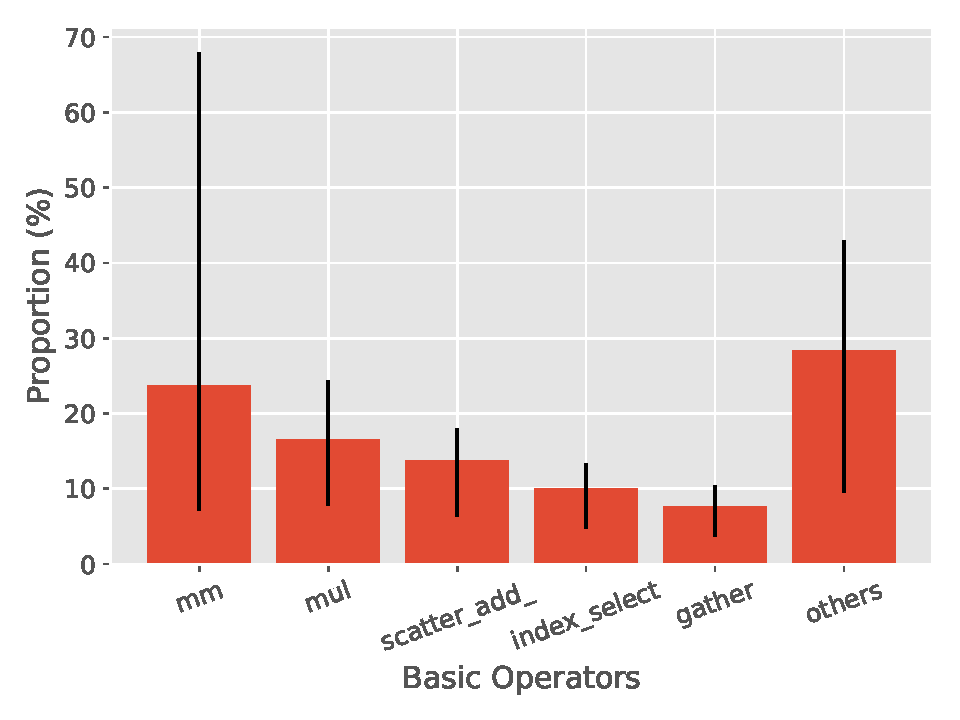
\includegraphics[height=4cm]{figs/experiments/exp_top_basic_ops_gcn.pdf}}
    \subfloat[GGNN]{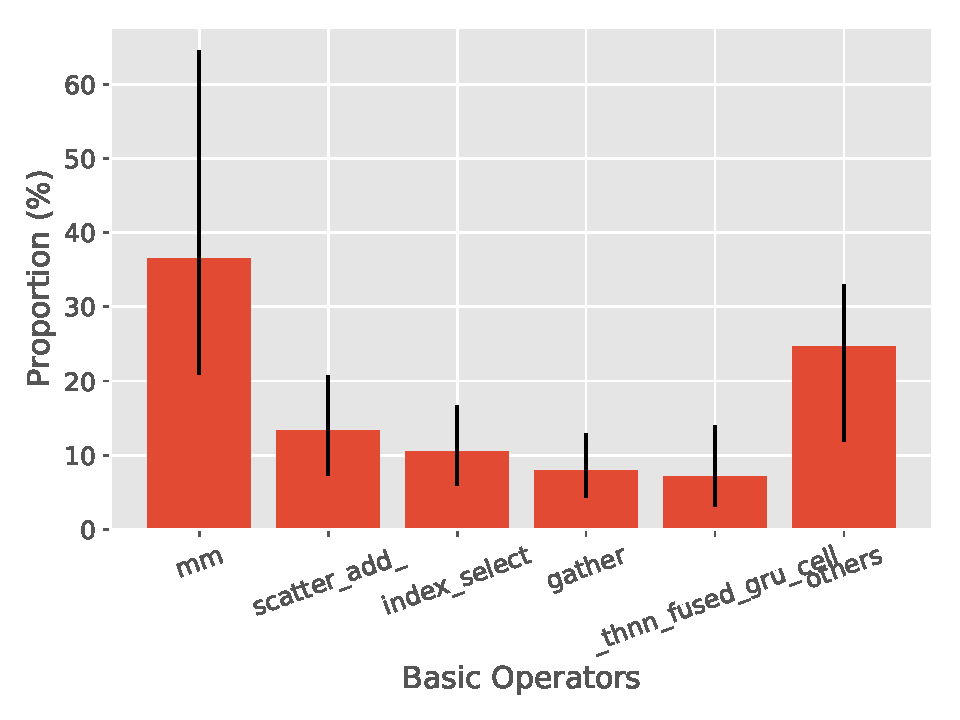
\includegraphics[height=4cm]{figs/experiments/exp_top_basic_ops_ggnn.pdf}}\\
    \subfloat[GAT]{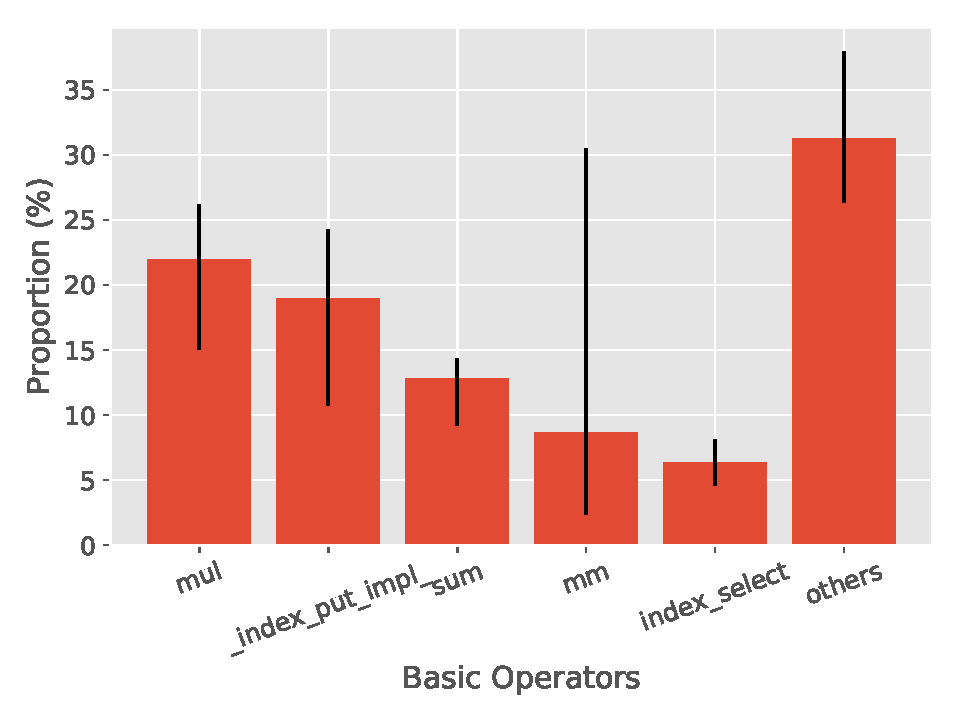
\includegraphics[height=4cm]{figs/experiments/exp_top_basic_ops_gat.pdf}}
    \subfloat[GaAN]{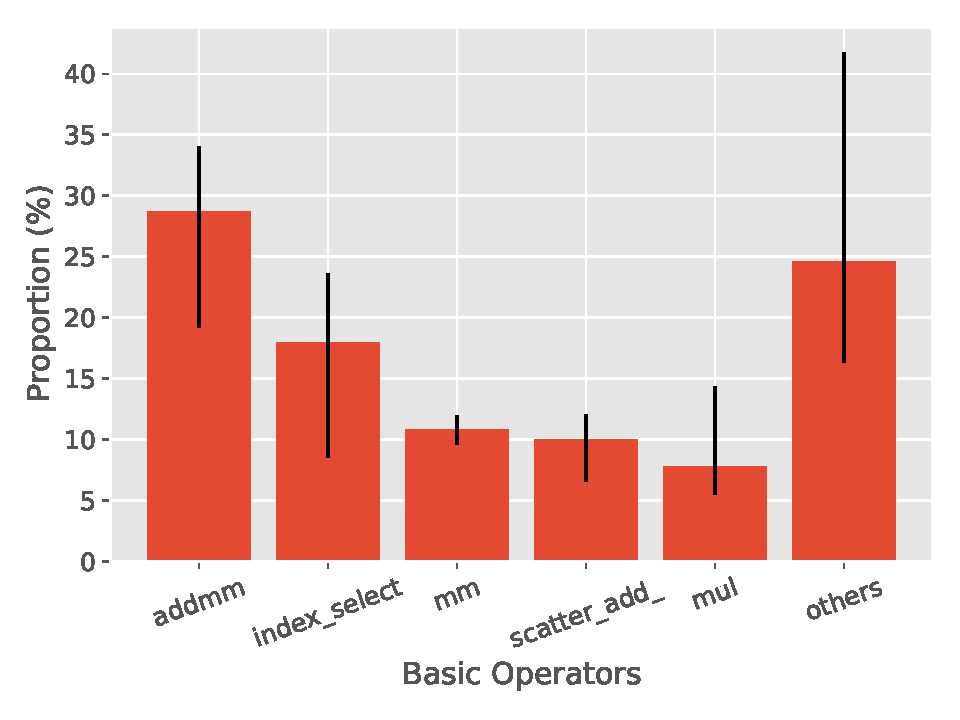
\includegraphics[height=4cm]{figs/experiments/exp_top_basic_ops_gaan.pdf}}
    \caption{Top 5 time-consuming basic operators of typical GNNs. The time proportion of each basic operator is averaged over all graphs with the error bar indicating the maximal and the minimal.}
    \label{fig:exp_top_basic_ops}
\end{figure}

\paragraph{GCN}
The most time-consuming basic operator was the matrix multiplication \texttt{mm} used in the vertex update function $\gamma$.
The elementwise multiplication \texttt{mul} used in the message function $\phi$ was also time-consuming.
The other three operators were used in the edge calculation: \texttt{scatter\_add\_} for the aggregation step in the forward phase, \texttt{gather} for the aggregation step in the backward phase, and \texttt{index\_select} for the collect step.
For GCN, the basic operators related to the edge calculation consumed the majority of the training time.

\paragraph{GGNN}
The top basic operator was \texttt{mm} used in the vertex calculation.
Due to the high time complexity in $\gamma$, the proportion of the \texttt{mm} operator were much higher than the other operators.
The \texttt{thnn\_fused\_gru\_cell} operator that was used in the backward phase of $\gamma$ was also noticeable.
The other three operators were used in the edge calculation.

\paragraph{GAT}
All the top basic operators except for \texttt{mm} were related to the edge calculation.
The \texttt{mm} operator was used in the vertex update function $\gamma$.

\paragraph{GaAN}
The top basic operator was \texttt{addmm}.
The \texttt{addmm}, the matrix multiplication \texttt{mm} and the elementwise multiplication \texttt{mul} were used in both the vertex and the edge calculation, where the edge calculation is dominant.

In general, the most time-consuming operator in GNN calculation is still the matrix multiplication \texttt{mm} and the elementwise multiplication \texttt{mul}, \emph{making GNN training suitable for GPU}.
Although the aggregate step in the edge calculation is relatively simple (like sum and mean), the related operators \texttt{scatter\_add} and \texttt{gather} still consumed a certain amount of the time.
They have to synchronize between hardware threads to avoid updating the same aggregated vector at the same time and they conducted non-regular memory access with the access pattern determined by the edge set dynamically.
For GPU, they were less efficient than \texttt{mm}.
The index-based selection \texttt{index\_select} operator from the collection step consumed around 10\% of time in all GNNs.
Though GPUs have high on-chip memory bandwidth, improving the efficiency of \texttt{scatter\_add}/\texttt{gather}/\texttt{index\_select} (like overlapping them with $\phi$) can benifit the training of all kinds of GNNs.

\paragraph{Summary}
The GNN training is suitable for GPU.
The \textbf{edge calculation is the main performance bottleneck}, except for training GNNs with high vertex calculation complexity on low-average-degree graphs.
The performance bottleneck in the edge calculation depends on the time complexity of the message function $\phi$.
\begin{itemize}
    \item If the time complexity of $\phi$ is \textbf{high}, the \textbf{efficiency of $\phi$} limits the performance. Reducing its computation cost (via optimizing its implementation or modifying the algorithm) can significantly reduce the training time.
    \item If the time complexity of $\phi$ is \textbf{low}, the \textbf{collect step} and the \textbf{aggregation step} limit the performance. The collect step involves lots of data movement. The aggregation step suffers from the data synchronization and non-regular data access. Optimizing their implementations can significantly reduce the training time.
\end{itemize}

\subsection{Memory Usage Analysis}
\label{sec:memory_usage_analysis}

During the GNN training, all data (including datasets and intermediate results) are stored in the on-chip memory of GPU.
Compared with the main memory on the host side, the capacity of the GPU memory is very limited.
\emph{The GPU memory capacity limits the scale of graphs that a GPU can train GNNs on}.
For example, GaAN was unable to complete the training due to memory overflow exception on \texttt{cph} dataset.

\begin{figure}
    \centering
    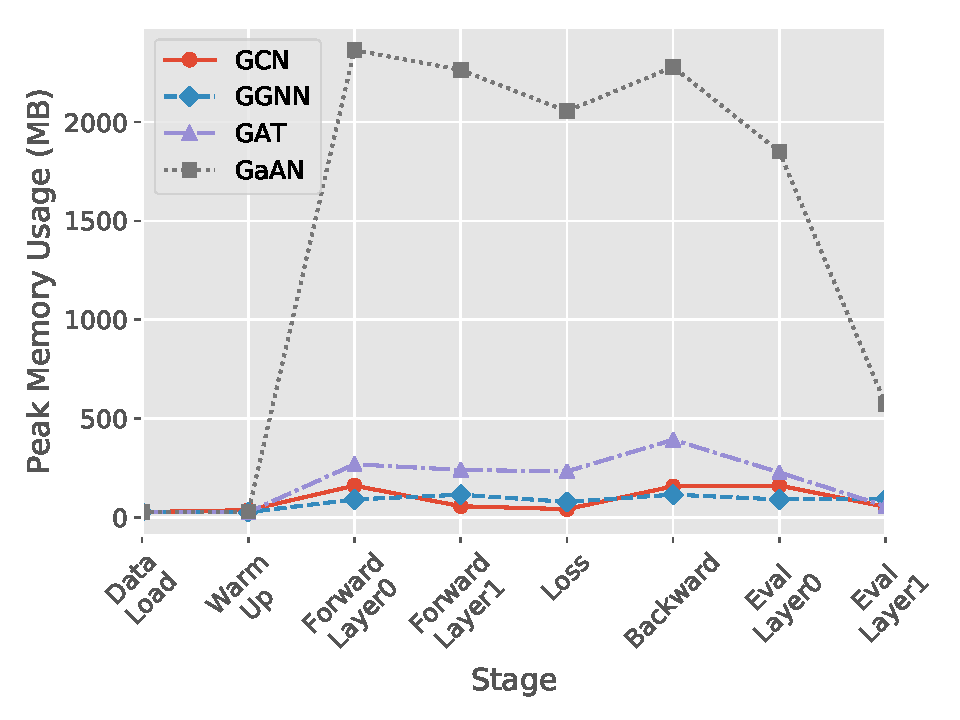
\includegraphics[height=5cm]{figs/experiments/exp_memory_usage_stage_amp.pdf}
    \caption{Memory usage of each phase. Dataset: \texttt{amp}.}
    \label{fig:exp_memory_usage_stage_amp}
\end{figure}

\begin{figure}
    \centering
    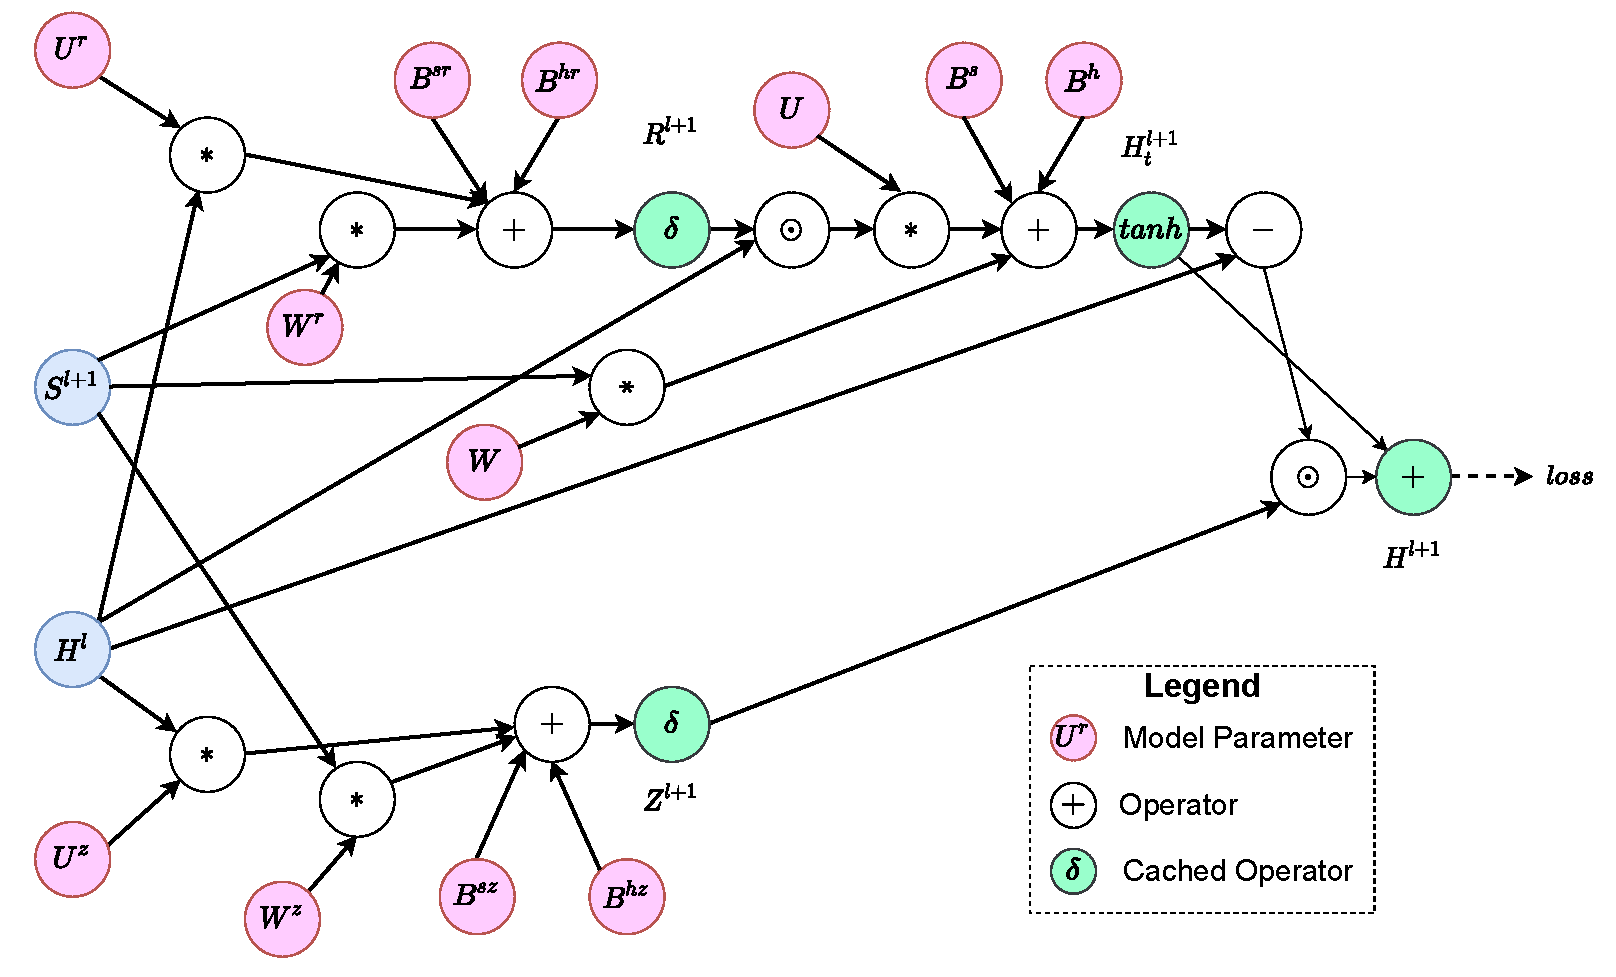
\includegraphics[height=4.5cm]{figs/illustration/ggnn_vertex_func_computation_graph.pdf}
    \caption{Computation graph of the vertex update function $\gamma$ of GGNN.}
    \label{fig:ggnn_vertex_func_computation_graph}
\end{figure}

\figurename~\ref{fig:exp_memory_usage_stage_amp} shows the peak memory usage of each phase in the GNN training on the \texttt{amp} dataset.
The trend was similar on other datasets.
\emph{The GNN training achieved its peak memory usage in the forward and the backward phases}.
The forward phase generated a large number of intermediate results.
Some key intermediate results were cached, increasing the memory usage.
The cached results were used in the gradient calculation in the backward phase.
\figurename~\ref{fig:ggnn_vertex_func_computation_graph} shows the computation graph of the vertex update function $\gamma$ of GGNN.
The computation graph had a large number of operators, each operator generating an intermediate matrix.
Some key intermediate matrices were cached.
The cached matrices were the main source of memory usage in the loss phase.
By the end of the backward phase, the cached results were released.
Since the evaluation phase did not need to calculate the gradients, it did not cache intermediate results.
Its memory usage declined sharply.

\begin{figure}
    \centering
    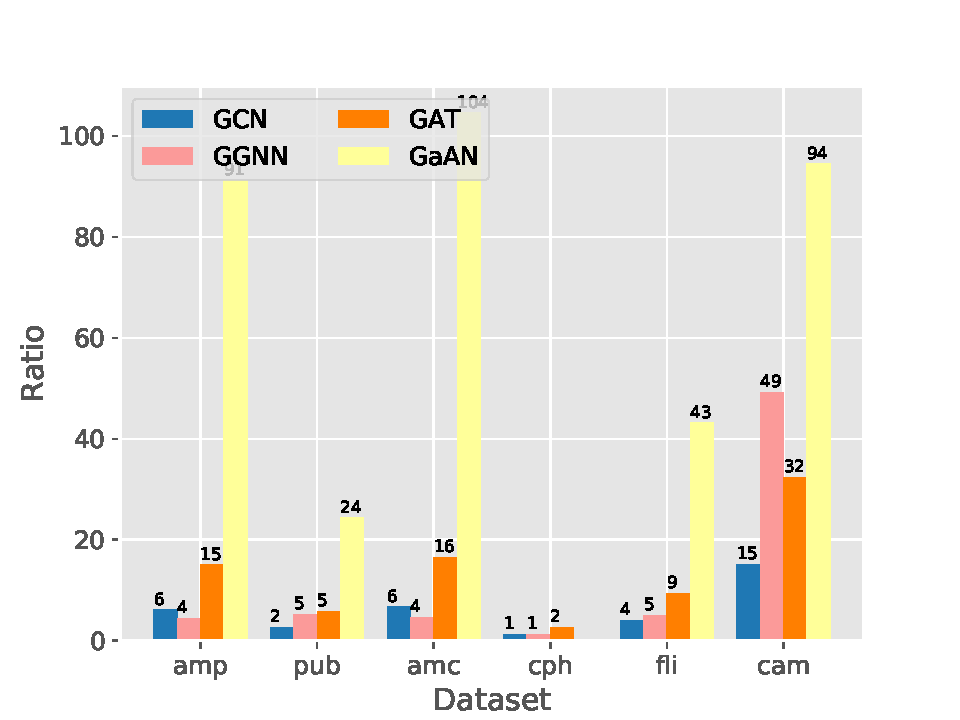
\includegraphics[height=5cm]{figs/experiments/exp_memory_expansion_ratio.pdf}
    \caption{Memory expansion ratios of typical GNNs.}
    \label{fig:exp_memory_expansion_ratio}
\end{figure}

The peak memory usage during the GNN training far exceeds the size of the dataset itself.
We define the \emph{memory expansion ratio} (MER) as the ratio of the peak memory usage during the training to the memory usage after loading the dataset.
\figurename~\ref{fig:exp_memory_expansion_ratio} compares MER of different GNNs.
GCN had the lowest MER (up to 14) while GaAN had the highest MER (up to 101).
\emph{The high MER limits the data scalability of GNNs}, making GPU unable to handle big graphs.

\begin{figure}
    \centering
    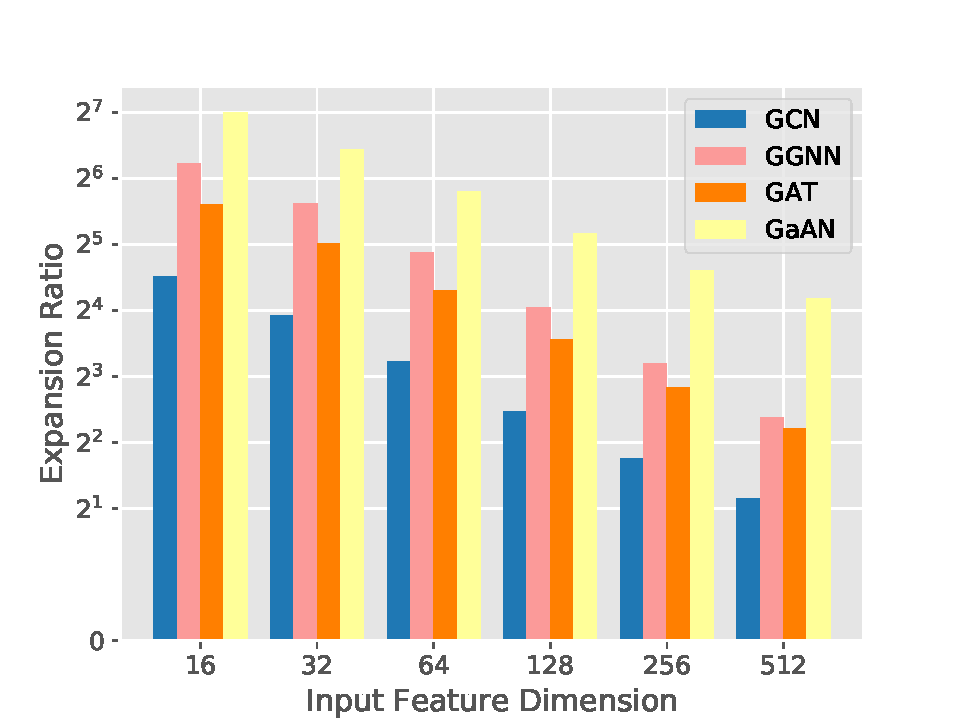
\includegraphics[height=5cm]{figs/experiments/exp_memory_expansion_ratio_input_feature_dimension_com-amazon.pdf}
    \caption{Memory expansion ratio under different dimensions of the input feature vectors. Dataset: \texttt{cam}.}
    \label{fig:exp_memory_expension_ratio_input_feature_dimension}
\end{figure}

\figurename~\ref{fig:exp_memory_expansion_ratio} also indicates that the same GNN had different MERs for different datasets.
Two characteristics of the dataset affects the MER: the dimension of the input feature vector and the average degree.

Given the same graph, the scales of the intermediate results are mainly affected by the hyper-parameters of the GNN.
If the dimension of the input feature vectors is high (like the \texttt{cph} dataset), the size of the dataset is large.
The size becomes comparable to the scales of the intermediate results,  making the MER low.
To find out how the dimension affects the MER, we generated random input feature vectors with different dimensions for the \texttt{cam} dataset and measured the MER in \figurename~\ref{fig:exp_memory_expension_ratio_input_feature_dimension}.
For a GNN under the same hyper-parameters, \emph{the MER decreased as the dimension of the input feature vectors increased}.

\begin{figure}
    \centering
    \subfloat[Peak memory usage]{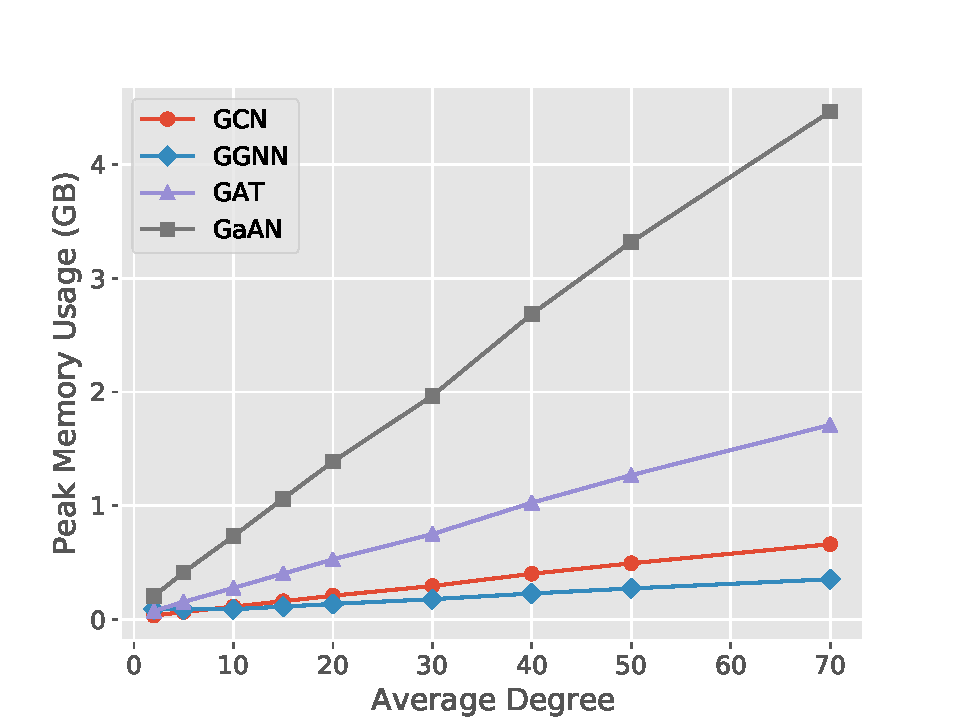
\includegraphics[height=4cm]{figs/experiments/exp_memory_expansion_ratio_input_graph_number_of_edges_peak_memory.pdf}}
    \subfloat[Memory expansion ratio]{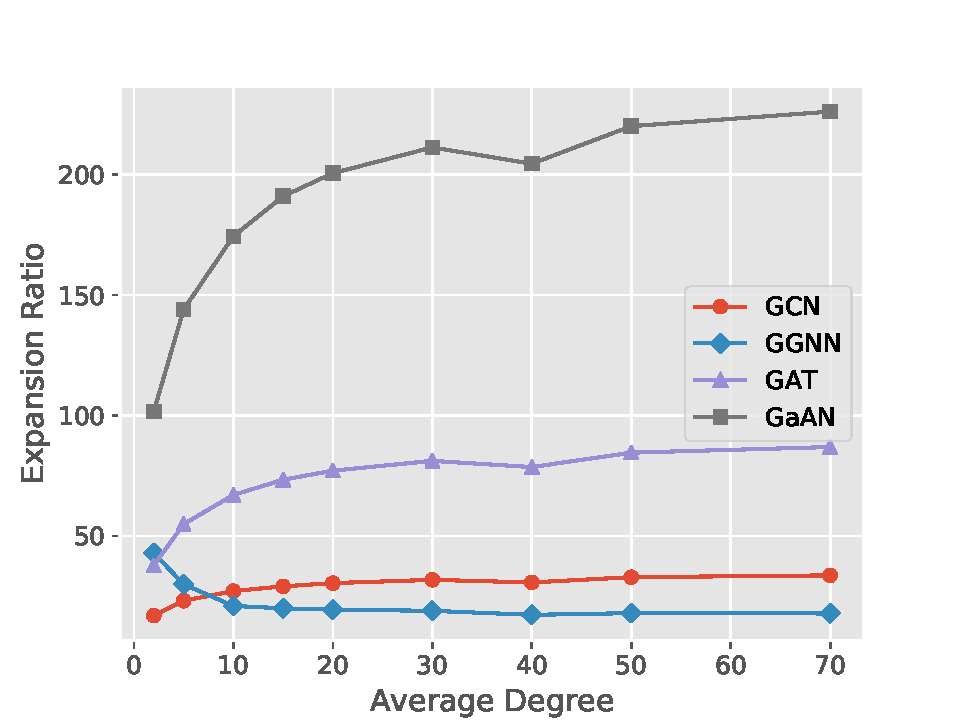
\includegraphics[height=4cm]{figs/experiments/exp_memory_expansion_ratio_input_graph_number_of_edges_expansion_ratio.pdf}}
    \caption{Memory usage under different average degrees of the graph. The graph was generated with the R-MAT generator fixing the number of vertices at 10K and the dimension of the input feature vectors at 32.}
    \label{fig:exp_memory_expansion_ratio_input_graph_number_of_edges}
\end{figure}

The average degree of the graph also affects MER by influencing the relative scale of the intermediate results from vertex/edge calculation.
Fixing the number of vertices $|\mathcal{V}|$, we used the R-MAT generator to generate random graphs with different average degrees.
\figurename~\ref{fig:exp_memory_expansion_ratio_input_graph_number_of_edges} shows how the memory usage changes according to the average degrees.
As the average degree $\bar{d}$ increased, the number of edges $|\mathcal{E}|$ increased and the peak memory usage increased \emph{linearly} with $\bar{d}$.
The edge calculation gradually dominated the memory usage and \emph{the MER converged to a stable value}.
The stable value was determined by the complexity of the edge calculation.
Except for GGNN, the MERs of the other GNNs increased as $\bar{d}$ increased.
As GGNN had high vertex calculation complexity, the MER related to the vertex calculation was much larger than the edge calculation.
When the edge calculation dominated the memory usage, its MER became smaller.

\begin{figure}
    \centering
    \subfloat[Peak memory usage]{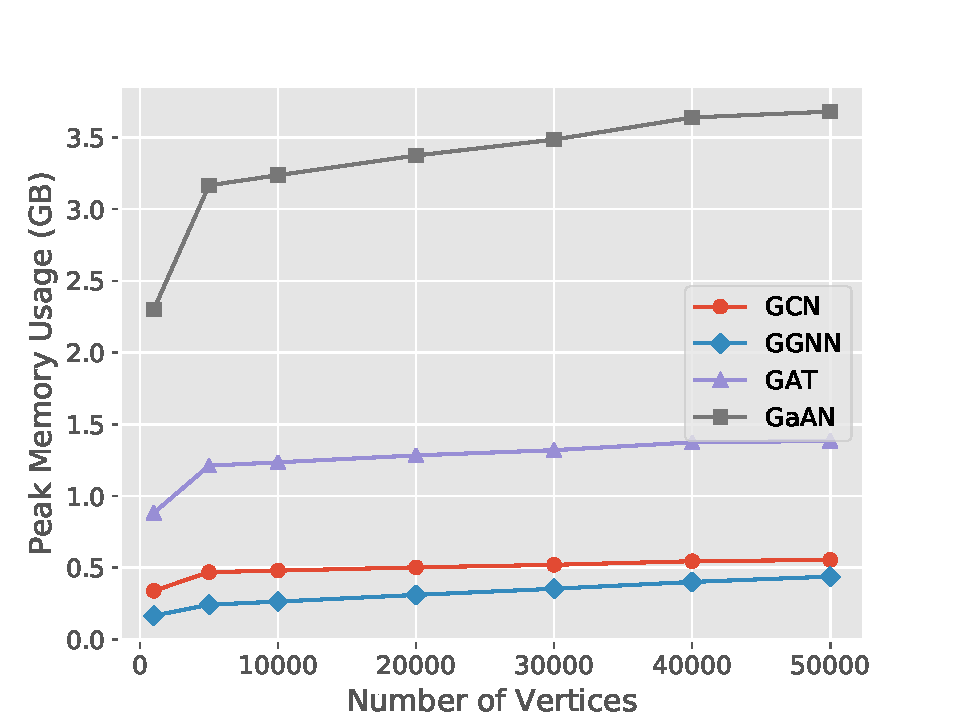
\includegraphics[height=4cm]{figs/experiments/exp_memory_expansion_ratio_input_graph_number_of_vertices_fixed_edge_peak_memory.pdf}}
    \subfloat[Memory expansion ratio]{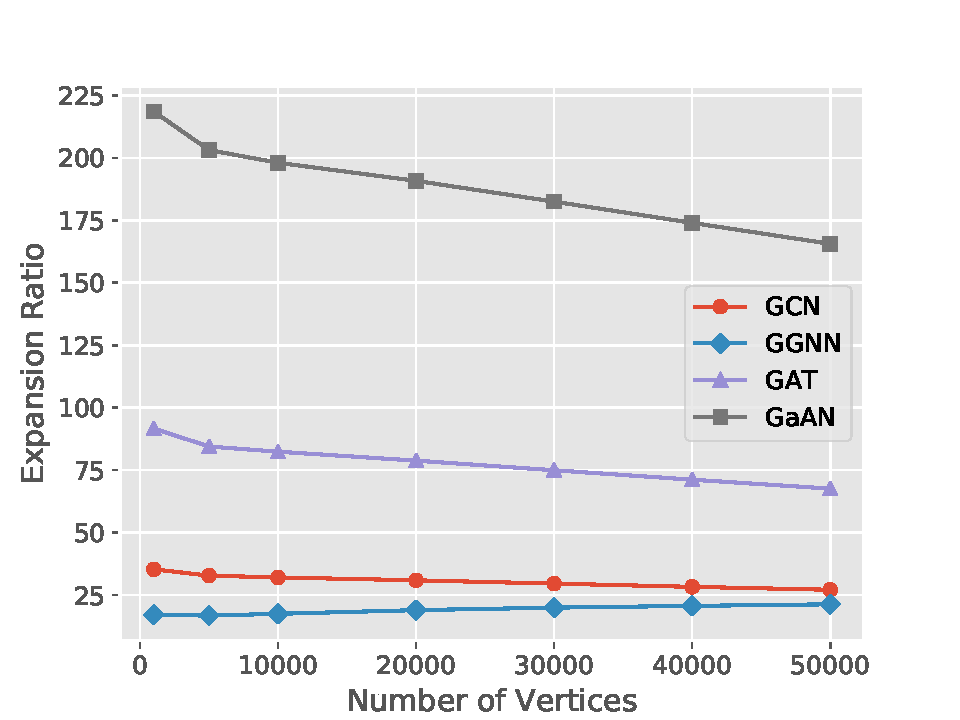
\includegraphics[height=4cm]{figs/experiments/exp_memory_expansion_ratio_input_graph_number_of_vertices_fixed_edge_expansion_ratio.pdf}}
    \caption{Memory usage under different numbers of vertices of the graph. The graph was generated with the R-MAT generator fixing the number of edges at 500K and the dimension of the input feature vectors at 32.}
    \label{fig:exp_memory_expansion_ratio_input_graph_number_of_vertices_fixed_edge}
\end{figure}

We also fixed the number of edges $|\mathcal{E}|$ in the graph and generated random graphs with different $|\mathcal{V}|$.
\figurename~\ref{fig:exp_memory_expansion_ratio_input_graph_number_of_vertices_fixed_edge} shows how the memory usage changed according to $|\mathcal{V}|$.
All GNNs were much more insensitive to the changes in $|\mathcal{V}|$ compared to $|\mathcal{E}|$.
Except for GGNN, the MERs of the other GNNs declined as $|\mathcal{V}|$ increased because the scale of the dataset increased quicklier than the scales of the intermediate results.
As GGNN had high vertex calculation complexity, the scales of the intermediate results were much more sensitive to $|\mathcal{V}|$.
It indicates that \emph{the intermediate results of the edge calculation dominated the memory usage during the GNN training}.

\paragraph{Summary}
The \emph{high} memory expansion ratio severely restricted the data scalability of the GNN training.
The memory usage mainly came from the intermediate results of the \emph{edge calculation}.
Fixing the number of vertices, the memory usage increased \emph{linearly} along with the number of edges.
Optimizing the memory usage of the edge calculation could significantly reduce the memory expansion ratio.
Fixing the GNN structure and the hyper-parameters, increasing the dimension of the input feature vectors could also reduce the memory expansion ratio.

\subsection{Effects of Sampling Techniques on Performance}
\label{sec:effects_of_sampling_techniques_on_performance}

With the sampling techniques, GNNs can be trained in a mini-batch manner.
Each mini-batch updates the model parameters based on a small subgraph sampled from the original input graph.
Thus, the training time per batch and the peak memory usage during the training should both decline significantly.

In the implementation in PyG, the GNN model and the dataset resided on the GPU side.
To process each epoch, PyG sampled the original dataset in the main memory and generated several batches.
Each batch was a small subgraph of the dataset.
To train on each batch, PyG sent the sampled subgraph to GPU, calculated the gradients in the subgraph and updated the model parameters directly on GPU.
With the sampling techniques, the model parameters were updated by a stochastic gradient descent optimizer.
It conducted the evaluation phase every several epoches (either on the CPU side or the GPU side) to determine whether to stop the training.
The experiments focused on the training phase of each batch.

\begin{figure}
    \centering
    \subfloat[Neighbor sampler]{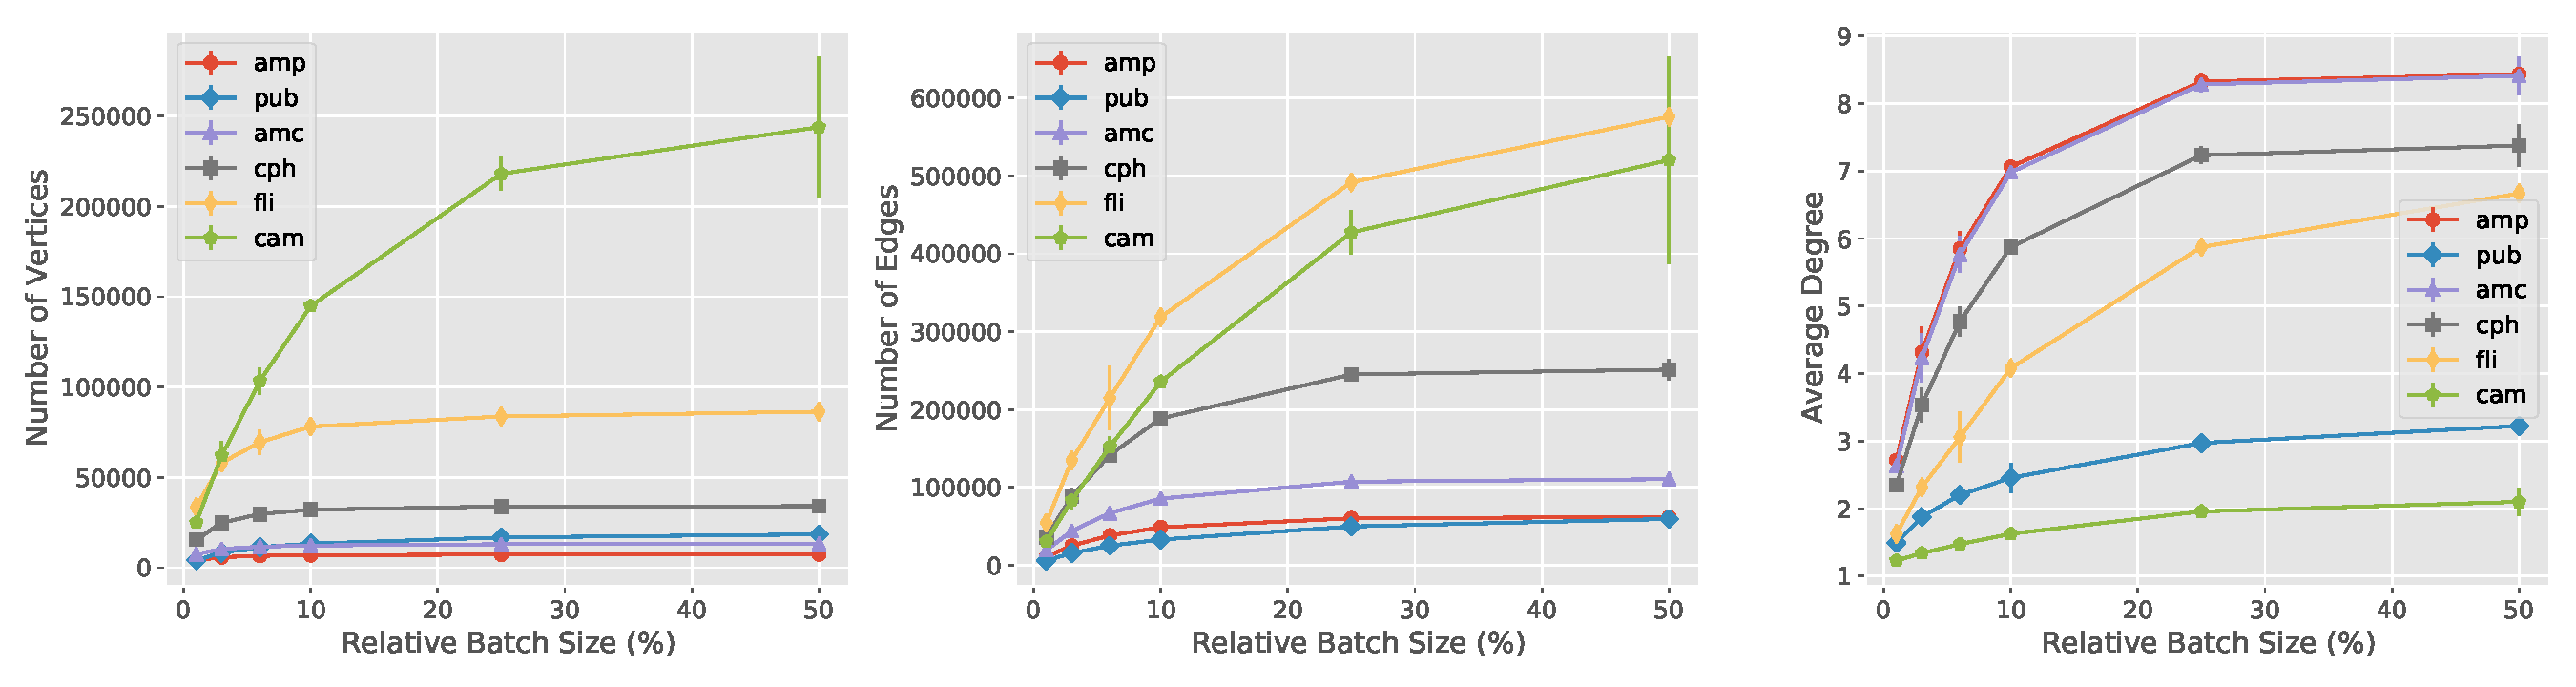
\includegraphics[height=4cm]{figs/experiments/exp_sampling_minibatch_realtive_graph_info_graphsage_gcn.pdf}} \\
    \subfloat[Cluster sampler]{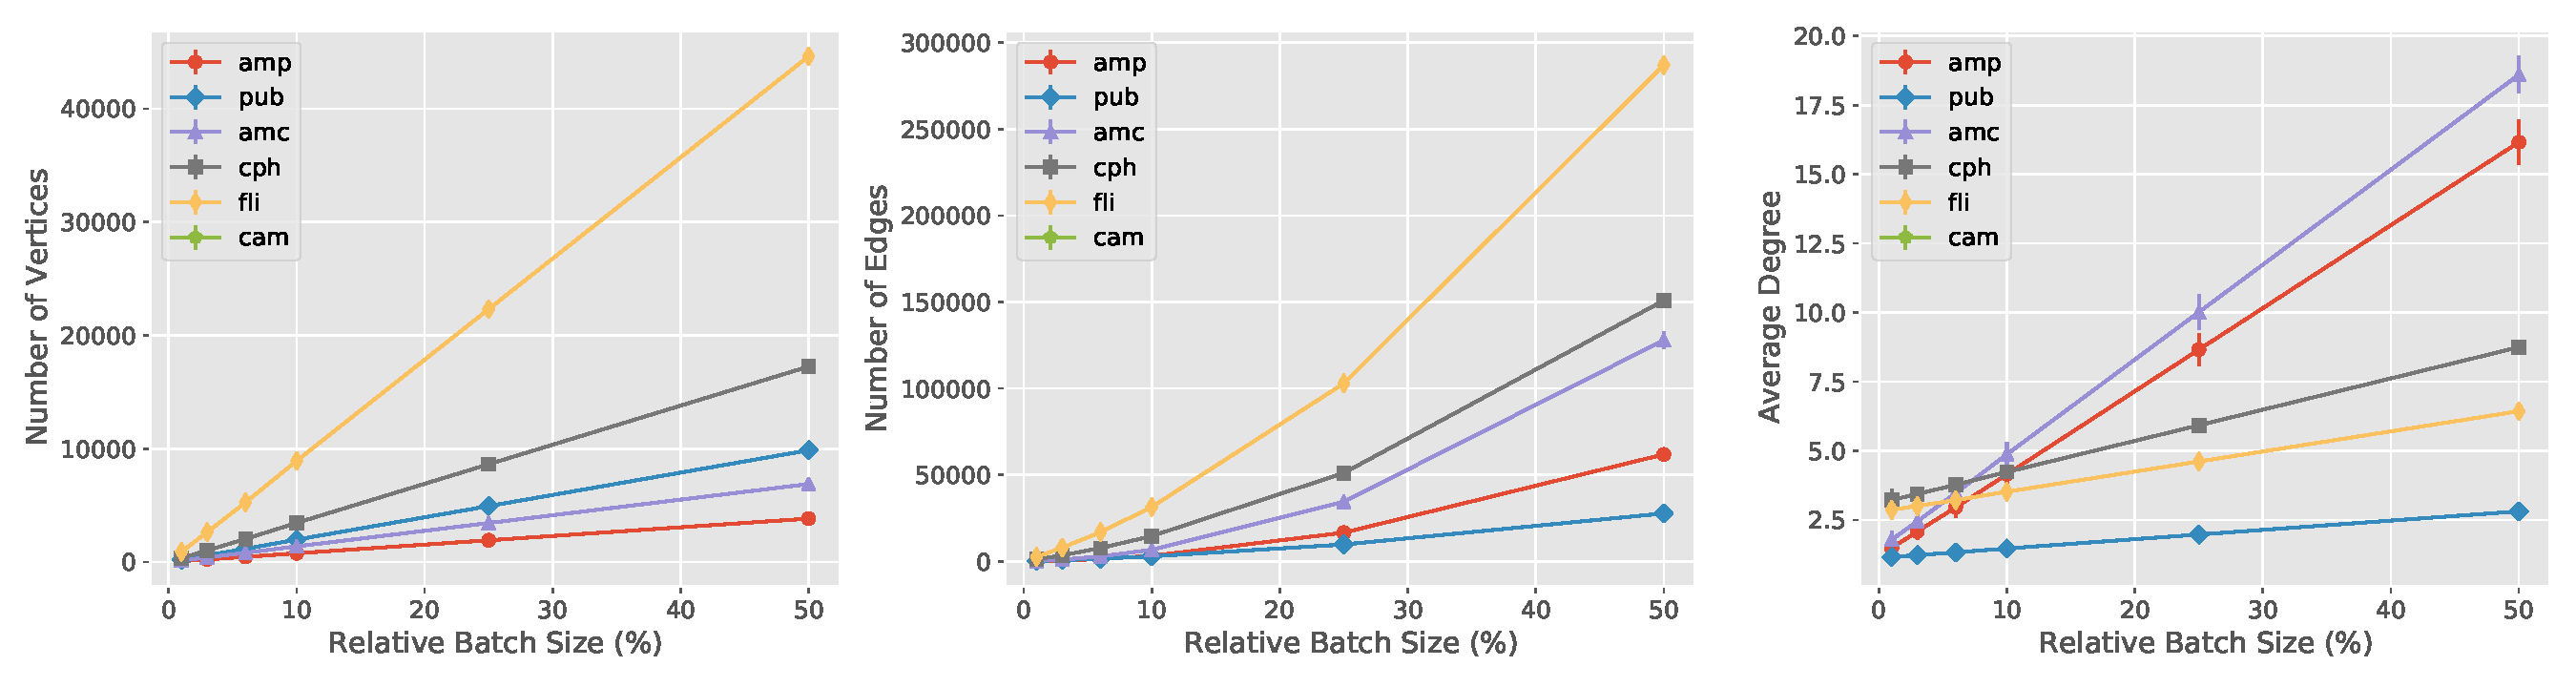
\includegraphics[height=4cm]{figs/experiments/exp_sampling_minibatch_realtive_graph_info_cluster_gcn.pdf}}
    \caption{Sizes of the sampled subgraphs under different batch sizes. Each batch size was sampled 50 times and the average value was reported. The error bar indicates the standard deviation. The batch size is relative to the full graph.}
    \label{fig:exp_sampling_minibatch_graph_info}
\end{figure}

\figurename~\ref{fig:exp_sampling_minibatch_graph_info} shows how the size of the sampled subgraph changed with the batch size.
For the neighbor sampler, the relative batch size is the porportion of the sampled vertices of the last GNN layer in all vertices of the graph.
For the cluster sampler, the relative batch size is the proportion of the sampled partitions to all partitions of the graph.
The neighbor sampler was very sensitive to the batch size.
As the batch size increased, the size of the sampled subgraph increased quickly and then stabalized.
The cluster sampler was much less sensitive compared to the neighbor sampler.
The number of vertices and the average degree of the sampled subgraphs increased linearly with the batch size.

\begin{figure}
    \centering
    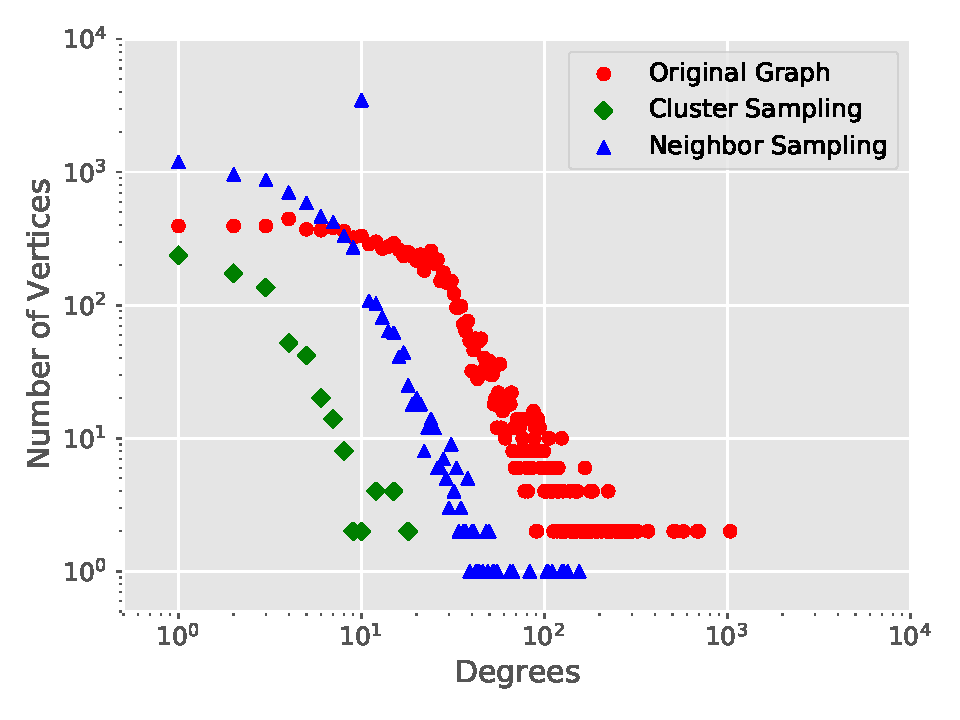
\includegraphics[width=0.4\columnwidth]{figs/experiments/exp_sampling_minibatch_degrees_distribution_amazon-photo.pdf}
    \caption{Vertex degree distribution of the sampled subgraph (relative batch size: 6\%) and the original graph. Dataset:\texttt{amp}.}
    \label{fig:exp_sampling_minibatch_degrees_distribution}
\end{figure}

It is worth noting that the average degree of the sampled subgraph was \emph{much lower} than the average degree of the whole graph, especially when the relative batch size is low.
Taking the neighbor sampler with the relative batch size of 6\% as an example, the average degree of the \texttt{amp} dataset was 31.1, but the average degree of the sampled subgraph was only 5.8.
For the cluster sampler, it was even lower to 3.0.
\figurename~\ref{fig:exp_sampling_minibatch_degrees_distribution} compares the degree distribution of the sampled subgraph with the original graph.
The slopes of the curves were similar.
It indicates that the sampled subgraphs still followed the power-law degree distribution.
However, the numbers of vertices in the sampled subgraphs were much smaller than the original graph, significantly lowering the average degrees.
According to the experimental results in Section~\ref{sec:training_time_breakdown}, if the average degree becomes lower, the proportion of the training time spent on vertex calculation will become higher, especially for GGNN.

\begin{figure}
    \centering
    \subfloat[Neighbor sampler on \texttt{amc}]{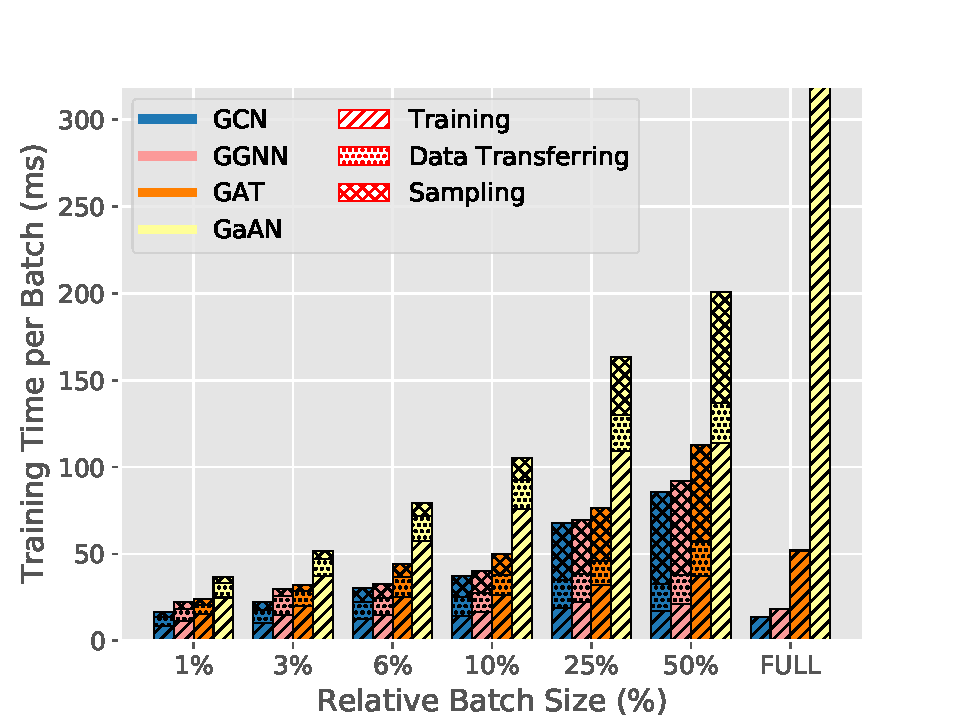
\includegraphics[height=5cm]{figs/experiments/exp_sampling_relative_batch_size_train_time_stack_graphsage_amazon-computers.pdf}}
    \subfloat[Neighbor sampler on \texttt{fli}]{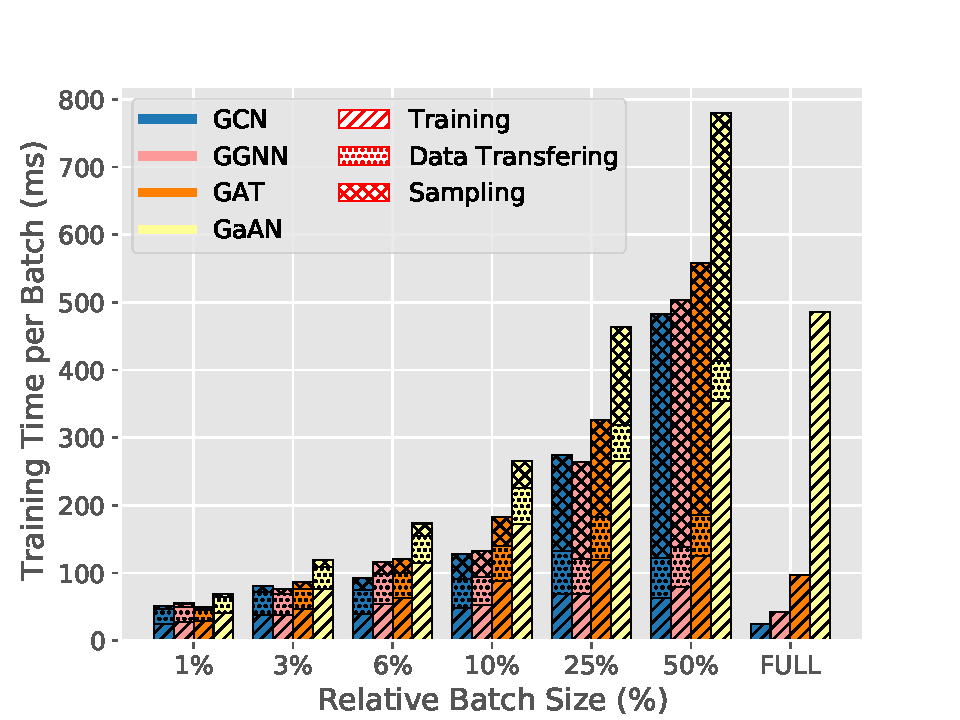
\includegraphics[height=5cm]{figs/experiments/exp_sampling_relative_batch_size_train_time_stack_graphsage_flickr.pdf}} \\
    \subfloat[Cluster sampler on \texttt{amc}]{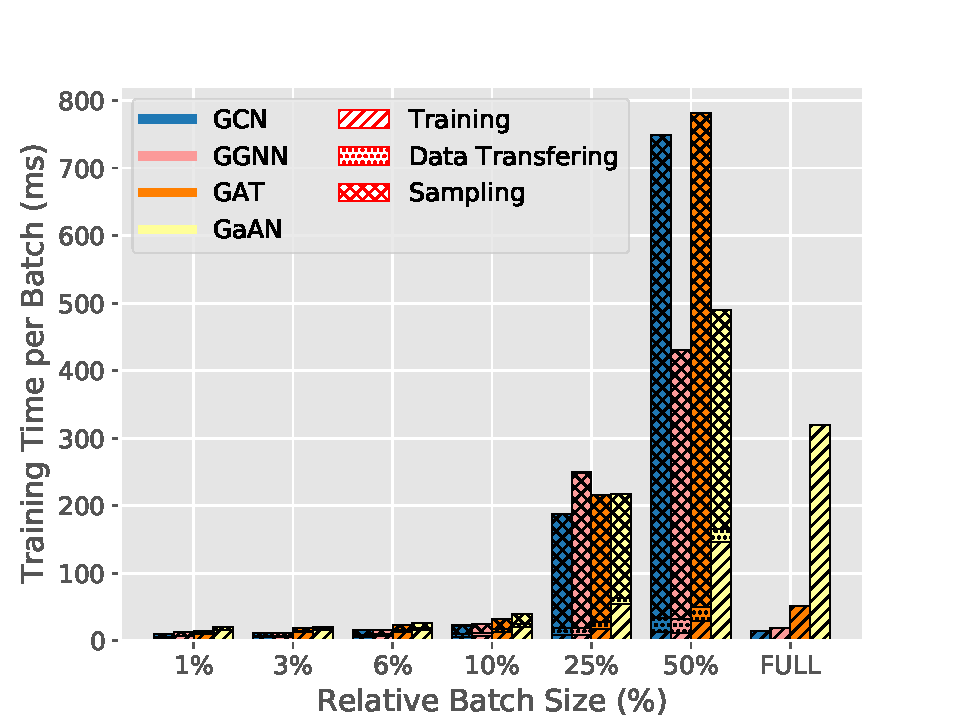
\includegraphics[height=5cm]{figs/experiments/exp_sampling_relative_batch_size_train_time_stack_cluster_amazon-computers.pdf}}
    \subfloat[Cluster sampler on \texttt{fli}]{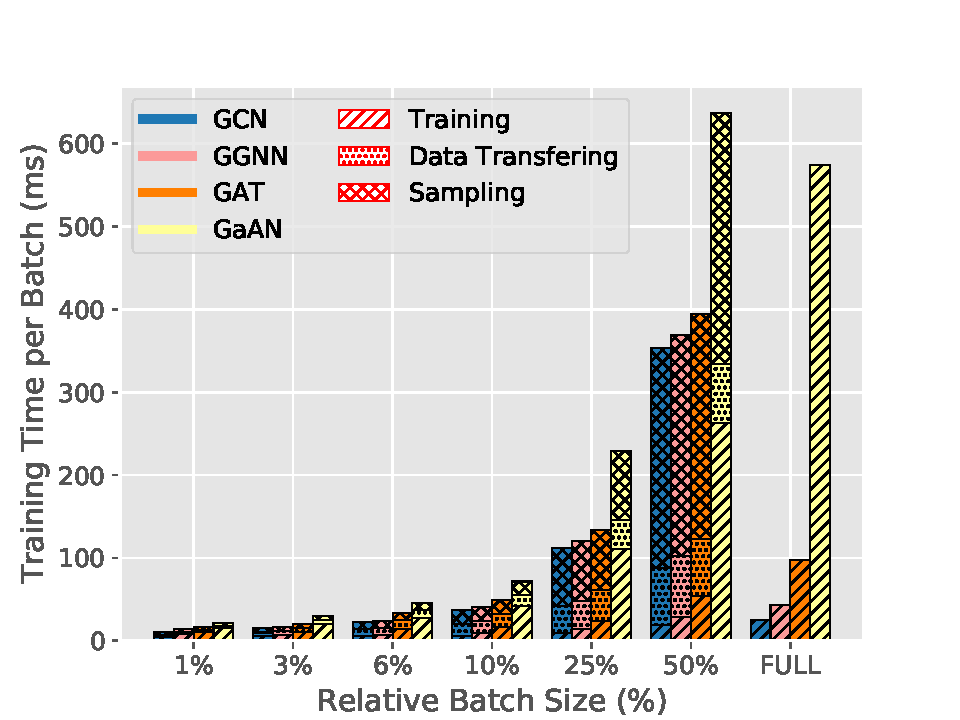
\includegraphics[height=5cm]{figs/experiments/exp_sampling_relative_batch_size_train_time_stack_cluster_flickr.pdf}}
    \caption{Training time per batch breakdown. FULL means that the full graph participates in the training.}
    \label{fig:exp_sampling_batch_train_time}
\end{figure}

To find out the performance bottleneck with the sampling techniques, we decomposed the training time per batch into three phases: \emph{sampling} on CPU, \emph{transfering} sampled subgraphs from CPU to GPU and \emph{training} with the subgraphs on GPU.
\figurename~\ref{fig:exp_sampling_batch_train_time} shows the time breakdown of the four GNNs under different relative batch sizes.
For the neighbor sampler, the sampling technique reduced the training time per batch only when the batch size was very small.
When the batch became bigger, the sampling and the data transfering phases introduced noticeable overheads, even making the training time exceed the full-batch training.
For the clustering sampler, the sampled subgraph was smaller than the neighbor sampler under the same relative batch size.
The reduction in the training time was more obvious than the neighbor sampler.
However, the overheads increased quickly as the relative batch size increased.
The training time under the 25\% relative batch size already exceeded the time of full-batch training.
The experimental results indicate that the implementation of the sampling techniques in PyG is inefficient.
When the batch size was slightly big, more than 50\% of the time had been spent on sampling and data transfering.
\emph{The sampling techniques are only efficient under small batch sizes.}

\begin{figure}
    \centering
    \subfloat[Neighbor sampler on \texttt{amc}]{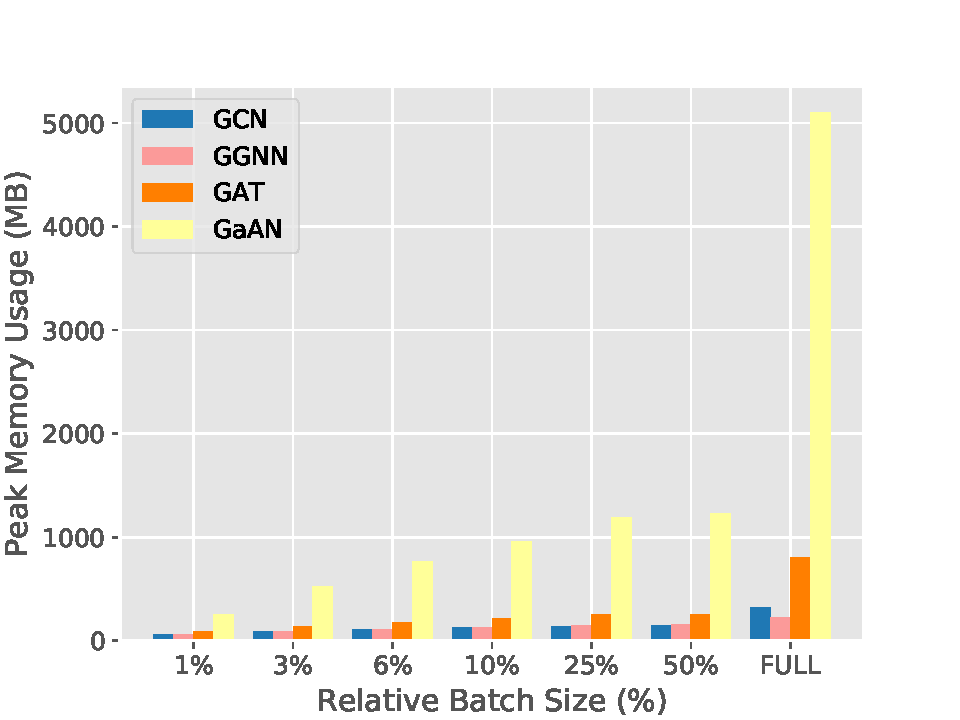
\includegraphics[height=4cm]{figs/experiments/exp_sampling_memory_usage_relative_batch_size_graphsage_amazon-computers_peak_memory.pdf}}
    \subfloat[Neighbor sampler on \texttt{fli}]{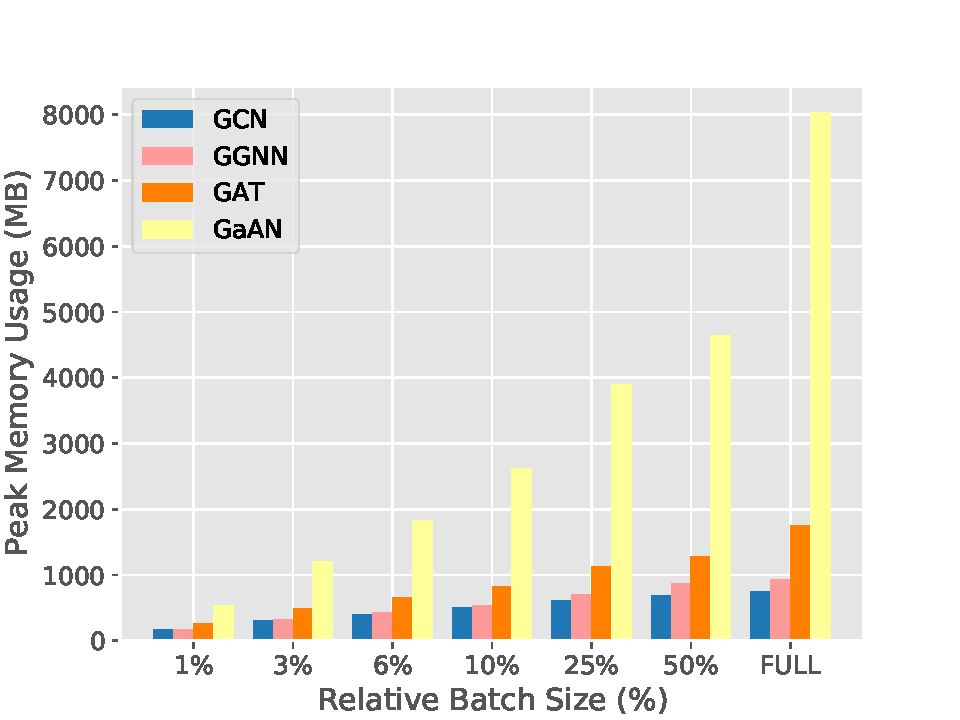
\includegraphics[height=4cm]{figs/experiments/exp_sampling_memory_usage_relative_batch_size_graphsage_flickr_peak_memory.pdf}} \\
    \subfloat[Cluster sampler on \texttt{amc}]{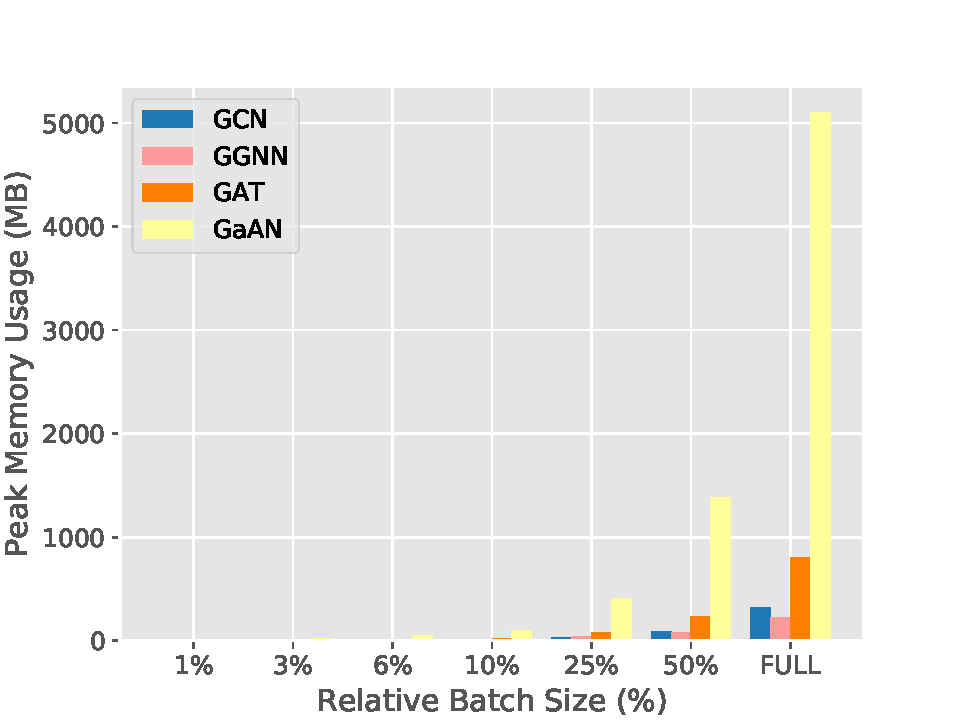
\includegraphics[height=4cm]{figs/experiments/exp_sampling_memory_usage_relative_batch_size_cluster_amazon-computers_peak_memory.pdf}}
    \subfloat[Cluster sampler on \texttt{fli}]{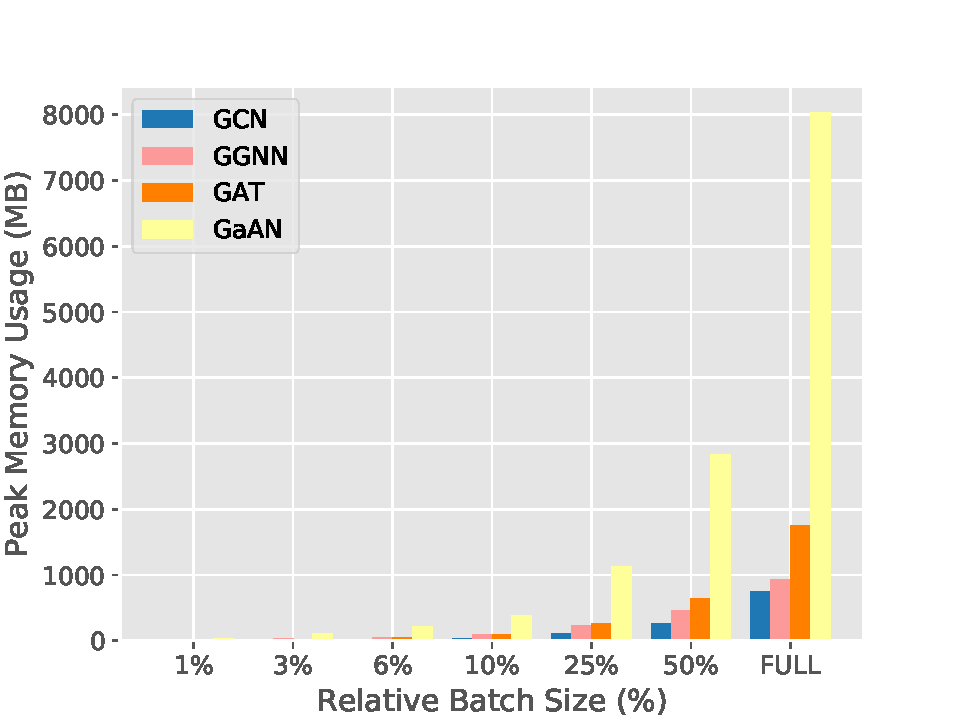
\includegraphics[height=4cm]{figs/experiments/exp_sampling_memory_usage_relative_batch_size_cluster_flickr_peak_memory.pdf}}
    \caption{Peak memory usage under different batch sizes. FULL means the full graph participates in the training.}
    \label{fig:exp_sampling_memory_usage}
\end{figure}

The main advantage of the sampling technique is \emph{reducing the peak memory usage} during the training.
\figurename~\ref{fig:exp_sampling_memory_usage} shows the memory usage under different batch sizes.
The peak memory usage declined significantly even under big batch sizes.
The sampling techniques make training GNNs on big graphs possible for GPU.

\paragraph{Summary}
With small batch size, the sampling techniques could significantly reduce the training time per batch and the peak memory usage during the training.
The sampled subgraphs had lower average degrees than the whole graph.
However, the current implementation of the sampling techniques was every inefficient under big batch sizes.
The time spent on the sampling phase and the data transfering phase could even exceeded the training phase.